\documentclass[11pt, fleqn]{article}
\usepackage[english]{babel}

\usepackage[lmargin=1.1in,rmargin=1.1in,bottom=1.3in,top=1.3in,
twoside=False]{geometry}

\usepackage{relsize,xspace}
 \usepackage{xcolor}
 \usepackage{mathtools}
 \usepackage{todonotes}
 \usepackage{comment}
\usepackage{microtype}
\usepackage{amsmath}
\usepackage{amssymb}
\usepackage{amsfonts}
\usepackage{stmaryrd}
\usepackage{bm}
\usepackage{tikz}
\usepackage{refcount}
\usepackage{wrapfig}

\usepackage{marginnote}


\definecolor{blue}{rgb}{0.1,0.2,0.5}
\definecolor{brown}{rgb}{0.6,0.6,0.2}
\usepackage[ocgcolorlinks, linkcolor={blue}, citecolor={brown}]{hyperref}

\usepackage[amsmath,thmmarks,hyperref]{ntheorem}
\usepackage{cleveref}


\crefformat{page}{#2page~#1#3}%
\Crefformat{page}{#2Page~#1#3}%
\crefformat{equation}{#2(#1)#3}%
\Crefformat{equation}{#2(#1)#3}%
\crefformat{figure}{#2Figure~#1#3}%
\Crefformat{figure}{#2Figure~#1#3}%
\crefformat{section}{#2Section~#1#3}
\Crefformat{section}{#2Section~#1#3}
\crefformat{chapter}{#2Chapter~#1#3}
\Crefformat{chapter}{#2Chapter~#1#3}
\crefformat{chapter*}{#2Chapter~#1#3}
\Crefformat{chapter*}{#2Chapter~#1#3}
\crefformat{part}{#2Part~#1#3}
\Crefformat{part}{#2Part~#1#3}
\crefformat{enumi}{#2(#1)#3}
\Crefformat{enumi}{#2(#1)#3}

\usepackage{enumerate}

\usepackage{latexsym}

% BEGIN ntheorem configuration

\theoremnumbering{arabic}
\theoremstyle{plain}
\theoremsymbol{}
\theorembodyfont{\itshape}
\theoremheaderfont{\normalfont\bfseries}
\theoremseparator{.}

\newtheorem{theorem}{Theorem}
\crefformat{theorem}{#2Theorem~#1#3}
\Crefformat{theorem}{#2Theorem~#1#3}
\renewcommand{\setminus}{-}
\newcommand{\newtheoremwithcrefformat}[2]{%
  \newtheorem{#1}[lemma]{#2}%
  \crefformat{#1}{##2\MakeUppercase#1~##1##3}%
  \Crefformat{#1}{##2\MakeUppercase#1~##1##3}%
}
\newcommand{\newseptheoremwithcrefformat}[2]{%
  \newtheorem{#1}{#2}%
  \crefformat{#1}{##2\MakeUppercase#1~##1##3}%
  \Crefformat{#1}{##2\MakeUppercase#1~##1##3}%
}

\newseptheoremwithcrefformat{lemma}{Lemma}
\newtheoremwithcrefformat{proposition}{Proposition}
\newtheoremwithcrefformat{observation}{Observation}
\newtheoremwithcrefformat{conjecture}{Conjecture}
\newtheoremwithcrefformat{corollary}{Corollary}
\newseptheoremwithcrefformat{claim}{Claim}
\theorembodyfont{\upshape}
\newtheoremwithcrefformat{example}{Example}
\newtheoremwithcrefformat{remark}{Remark}
\newseptheoremwithcrefformat{definition}{Definition}

\theoremstyle{nonumberplain}
\theoremheaderfont{\scshape}
\theorembodyfont{\normalfont}
\theoremsymbol{\ensuremath{\square}}
\newtheorem{proof}{Proof}

\theoremsymbol{\ensuremath{\lrcorner}}
\newtheorem{clproof}{Proof}

% END ntheorem configuration

\newcommand{\set}[1]{\{#1\}}
\renewcommand{\subset}{\subseteq}

%\setlength{\parskip}{0.1cm}
%\setlength{\parindent}{0cm}
%\setlength{\mathindent}{1cm}

\newcommand{\wcol}{\mathrm{wcol}}
\newcommand{\col}{\mathrm{col}}
\newcommand{\adm}{\mathrm{adm}}
\newcommand{\tw}{\mathrm{tw}}
\newcommand{\WReach}{\mathrm{WReach}}
\newcommand{\SReach}{\mathrm{SReach}}
\newcommand{\wcolorder}{\sqsubseteq}
\newcommand{\Oof}{\mathcal{O}}
\newcommand{\CCC}{\mathcal{C}}
\newcommand{\NNN}{\mathcal{N}}
\newcommand{\WWW}{\mathcal{W}}
\newcommand{\DDD}{\mathcal{D}}
\newcommand{\PPP}{\mathcal{P}}
\newcommand{\FFF}{\mathcal{F}}
\newcommand{\GGG}{\mathcal{G}}
\newcommand{\YYY}{\mathcal{Y}}
\newcommand{\nei}{\mathrm{nei}}
\renewcommand{\ker}{\mathrm{ker}}
\newcommand{\core}{\mathrm{core}}

\newcommand{\cutrk}{\mathrm{cutrk}}
\newcommand{\rank}{\mathrm{rank}}
\newcommand{\rw}{\mathrm{rw}}


\newcommand{\grad}{\nabla}
\newcommand{\ds}{\mathbf{ds}}
\newcommand{\cl}{\mathrm{cl}}
\newcommand{\cst}{\alpha}

\newcommand{\fnei}{f_{\nei}}
\newcommand{\fwcol}{f_{\wcol}}
\newcommand{\fker}{f_{\ker}}
\newcommand{\fproj}{f_{\mathrm{proj}}}
\newcommand{\fcl}{f_{\cl}}
\newcommand{\fgrad}{f_{\grad}}
\newcommand{\fpaths}{f_{\mathrm{pth}}}
\newcommand{\fapx}{f_{\mathrm{apx}}}
\newcommand{\fcore}{f_{\mathrm{core}}}
\newcommand{\ffin}{f_{\mathrm{fin}}}

\newcommand\blfootnote[1]{%
  \begingroup
  \renewcommand\thefootnote{}\footnote{#1}%
  \addtocounter{footnote}{-1}%
  \endgroup
}

\newcommand{\suchthat}{ \colon }
\newcommand{\sth}{ \colon }
\newcommand{\ie}{i.e.\@ }
\newcommand{\N}{\mathbb{N}}
\newcommand{\R}{\mathbb{R}}
\newcommand{\tup}[1]{\bar{#1}}
\renewcommand{\phi}{\varphi}
\renewcommand{\epsilon}{\varepsilon}
\newcommand{\str}{\mathfrak}
\newcommand{\strA}{\str{A}}
\newcommand{\strB}{\str{B}}
\newcommand{\FO}{\mathrm{FO}}
\newcommand{\minor}{\preccurlyeq}
\newcommand{\dist}{\mathrm{dist}}
\newcommand{\indx}{\mathrm{index}}
\renewcommand{\mid}{~:~}

\newcommand{\profnum}{\widehat{\nu}}
\newcommand{\projnum}{\mu}
\newcommand{\projprof}{\widehat{\mu}}

\newcommand{\abs}[1]{\ensuremath{\left\lvert#1\right\rvert}}

\newcommand{\im}{\mathrm{im}}
\newcommand{\rg}{\mathrm{rg}}
\newcommand{\from}{\colon}


\newcounter{aux}

\title{On Wideness and Stability
\thanks{
The work of M.\ Pilipczuk and S.\ Siebertz is supported by the National Science Centre of 
Poland via POLONEZ grant agreement UMO-2015/19/P/ST6/03998, 
which has received funding from the European Union's Horizon 2020 research and 
innovation programme (Marie Sk\l odowska-Curie grant agreement No.\ 665778).
M. Pilipczuk is supported by the Foundation for Polish Science (FNP) via the START stipend programme.
}}

\author{
Micha\l~Pilipczuk \qquad
\qquad Sebastian Siebertz
\qquad Szymon Toru{\'n}czyk\\[0.3cm]
Institute of Informatics, University of Warsaw, Poland\\[0.1cm]
\texttt{\{michal.pilipczuk,siebertz,szymtor\}@mimuw.edu.pl}}

\begin{document}

\maketitle

\begin{abstract}
\noindent 
Nowhere dense classes of graphs were introduced 
by Nešetřil and Ossona de 
Mendez~\cite{nevsetvril2010first,nevsetvril2011nowhere} as a model
for uniform sparseness of graphs. The concept of nowhere denseness
turns out to be very robust as witnessed by the fact that it is equivalent 
to multiple other concepts studied in different areas of mathematics. 
In this work we revisit the connections between the notion of nowhere 
denseness and notions from (finite) model theory.

Based on work of Podewski and Zieger~\cite{podewski1978stable}, 
Adler and Adler~\cite{adler2014interpreting}
proved that every nowhere dense class $\CCC$ of graphs is stable, that is, 
the ladder index of every first-order formula $\phi(\tup{x},\tup{y})$ over
graphs from $\CCC$ is bounded by a constant depending only on $\phi$ and
$\CCC$. The original proof of this fact is based on an infinite
Ramsey argument and explicit bounds on ladder indices were never given. 
We give a combinatorial proof of Adler and Adler's result in 
the finite and work out the explicit bounds for ladder indices of
first-order formulas on nowhere dense classes of graphs. 

A class $\CCC$ of graphs if uniformly quasi-wide if there are functions 
$N:\N\times\N\rightarrow\N$ and $s:\N\rightarrow\N$ such 
that for all $G\in \CCC$ and all $r,m\in \N$, if $A\subseteq V(G)$ is
of size at least $N(r,m)$ then there is a set $S$ of size at most $s(r)$
such that there is a subset $B\subseteq A\setminus S$ which is
$r$-independent in $G-S$. It was proved in~\cite{siebertz2016polynomial} 
that we can always choose $N(r,m)\leq m^{f(r)}$, for a function $f$ whose
existence follows from the earlier non-constructive argument of Podewski 
and Ziegler. We give a simpler proof of this result with much improved bounds 
on $f(r)$.

Finally, we observe that an argument of Bousquet and 
Thomasse\'e~\cite{BousquetT15} can be slightly modified to prove that 
the VC-dimension of the $r$-power graph $G^r$ of a graph $G$
with $K_t\not\minor_r G$ is bounded by $t-1$.
\end{abstract}

\begin{picture}(0,0) \put(445,-265)
{\hbox{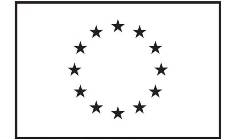
\includegraphics[scale=0.25]{flag_bw.jpg}}} \end{picture} 
\vspace{-0.8cm}

%\section{Introduction}

Nowhere dense classes of graphs were introduced 
by Ne\v set\v ril and Ossona de 
Mendez~\cite{nevsetvril2010first,nevsetvril2011nowhere} as a very 
general model
for uniform sparseness of graphs. These classes generalize many 
familiar classes of sparse graphs, such as planar graphs, graphs 
of bounded treewidth,  graphs of bounded degree, and, in fact, 
all classes that exclude a fixed 
topological minor.
The concept of nowhere denseness
turns out to be very robust as witnessed by the fact that it is equivalent 
to multiple other concepts studied in different areas of mathematics. 
One can equivalently characterize nowhere dense graph classes 
by bounds on the density of shallow (topological)
minors~\cite{nevsetvril2010first,nevsetvril2011nowhere},
quasi-wideness~\cite{nevsetvril2011nowhere} (a notion introduced by
Dawar~\cite{dawar2010homomorphism} in his study of homomorphism
preservation properties), low tree-depth
colorings~\cite{nevsetvril2008grad}, generalized coloring
numbers~\cite{zhu2009coloring}, sparse neighborhood
covers~\cite{GroheKRSS15,grohe2014deciding}, by a game called the
splitter game~\cite{grohe2014deciding} and by the model-theoretic
concepts of stability and independence~\cite{adler2014interpreting}.
For a broader discussion on the graph theoretic sparsity we refer to the book
of Ne\v{s}et\v{r}il and Ossona de Mendez~\cite{sparsity}.

These alternative characterizations have been very useful in 
the design of efficient algorithms. For instance, 
the {\sc{Subgraph Isomorphism}} and {\sc{Homomorphism}} problems 
are fixed-parameter tractable on any nowhere dense
class, parameterized by the size of the pattern graph~\cite{nevsetvril2010first}
and so is the {\sc Distance-$r$ Dominating Set} problem, parameterized
by the size of the solution~\cite{DawarK09}. In fact, 
the {\sc Distance-$r$ Dominating Set} problem admits
polynomial kernels~\cite{siebertz2016polynomial} and even 
almost linear kernels on nowhere dense classes of 
graphs~\cite{eickmeyer2016neighborhood}
(see also~\cite{drange2016kernelization} for the case $r=1$). 
It was shown in~\cite{grohe2014deciding}
that every first-order definable problem can be decided in
almost linear time on any nowhere dense graph class.

It is a natural question to ask for the most general classes of graphs
which admit efficient solutions for certain problems, or to 
classify them into tractable and intractable classes. It was shown 
that for the first-order model-checking problem~\cite{dvovrak2013testing} and for
the {\sc Distance-$r$ Dominating Set} problem~\cite{drange2016kernelization} 
the dividing line for algorithmic tractability 
on subgraph closed classes of graphs is exactly between the
nowhere dense and somewhere dense graph classes. 

\smallskip

In (infinite) model theory, we are a different classification program is followed. An important 
problem is to count the number and classify the models of a complete theory. According
to the upward L\"ownheim-Skolem theorem, every theory $T$ with an infinite model has
models of arbitrary infinite cardinalities (larger then the size of the language). One of the central problems
 is to determine, for any fixed infinite cardinal~$\kappa$, how many models of cardinality 
$\kappa$ the theory $T$ can have (up to isomorphism). Note that the number of
models of cardinality $\kappa$ must lie between $1$ and $2^\kappa$ for all infinite cardinals $\kappa$ 
bigger than the cardinality of the language. By a result of 
Morley~\cite{morley1965categoricity}, if $T$ is a countable
theory which has only one model of cardinality $\kappa$ for some uncountable $\kappa$, 
then $T$ has only one model for all uncountable cardinals; a result which 
is often considered the starting point of modern model theory. In his famous classification
project~\cite{shelah1990classification}, Shelah essentially provided a complete
classification for all countable theories (the classification was completed 
in~\cite{hart2000uncountable}). Shelah identified several dividing lines and showed that
all theories on the non-structure side of the dividing line have $2^\kappa$ models
of cardinality $\kappa$. On
the structure side he showed that there are only few models whose isomorphism 
types can be described by small invariants. One of the most important dividing 
lines is \emph{stability}. Very roughly, if a theory is not stable then its models 
are too many and too complicated to classify, while this may be possible if the theory is stable, 
especially if the theory is \emph{superstable} or \emph{totally transcendental}.

Finite model theory is the study of the expressive power 
of logics on the class of finite structures. Many theorems and 
methods of classical model theory fail when only finite structures 
are considered. These include the compactness theorem, the completeness 
theorem and various interpolation and preservation theorems.
On the other hand, quite different questions, which often arise in
computer science, in particular questions from complexity theory and database
theory, are interesting in finite model theory. Hence, instead of focusing 
on negative results, much work has been invested in finding 
subclasses of the class of all finite structures that may be better behaved.
Surprisingly, it turns out that particularly classes which are 
algorithmically well-behaved turn out to have good model-theoretic 
properties. The two prime examples in our context are the result of 
Dawar~\cite{dawar2010homomorphism}, who introduced the notion of
quasi-wideness and proved any quasi-wide class that is closed under taking substructures
and disjoint unions has the homomorphism preservation property. It was 
later proved by Ne\v{s}et\v{r}il and Ossona de Mendez that 
the notions of uniform quasi-wideness and nowhere denseness coincide for 
graphs~\cite{nevsetvril2011nowhere}. The second result is by 
Adler and Adler~\cite{adler2014interpreting}, who observed that 
nowhere denseness essentially corresponds to the stability theoretic notion 
of \emph{superflatness} introduced by Podewski and 
Ziegler in~\cite{podewski1978stable}. In fact, Adler and Adler observed 
that on subgraph closed classes of graphs, the notions of nowhere denseness, 
stability and the non-independence property (NIP) are equivalent. 
Before we can give an 
overview of some of the techniques that can be brought down from 
the infinite to the finite and state our contributions, we need some
definitions. 

\paragraph{Stability.}
We start from recalling some notions from stability theory. 



\begin{definition}
Let $\cal C$ be a class of structures in a first-order language $L$. Let 
$\phi(\tup{x},\tup{y})$ be an $L$-formula with the free variables
divided into two groups $\tup{x}, \tup{y}$. A \emph{$\phi$-ladder}
of length $n$ is a sequence $(\tup{a}_1,\ldots, \tup{a}_{n},
\tup{b}_1,\ldots, \tup{b}_{n})$ of tuples in some model $\strA\in \cal C$, such that for all $1\leq i,j\le n$,
\[\strA\models\phi(\tup{a}_i,\tup{b}_j)\Longleftrightarrow i\leq j. \]
The least  $n$ for which 
there is no $\phi$-ladder of length $n$ is 
the \emph{ladder index} 
of $\phi(\tup{x},\tup{y})$ in $\cal C$ (which may depend on the way we split the
variables).
A formula $\phi$ is \emph{stable} (for $\cal C$) if its ladder index is finite, and \emph{unstable} otherwise. The class of structures $\cal C$ is \emph{stable} if  every formula is stable.
\end{definition}

By abuse of notation, we will apply the above definition to a single structure $\strA$ in place of a class $\cal C$; formally, this amounts to considering the class $\cal C=\set\strA$.


Usually, in model theory one fixes a complete theory $T$
and takes as the class $\cal C$ above the class of all models of the theory $T$. The theory $T$ is then called stable if the class $\cal C$ is stable.
We remark that a formula with ladder index $n$ is said to have the
$n$-order property in~\cite{adler2014interpreting} and~\cite{ensley1996finite}.
We follow the notation of the textbook~\cite{hodges1993model} and remark
that it is easy to see that a class $\CCC$ is stable if and only if there is no 
formula $\psi(\tup{x},\tup{y})$ such that for every $n\in \N$
there exist a structure $\strA\in \CCC$ and tuples $\tup{a}_1,\ldots, \tup{a}_{n}$
of elements of $\strA$ such that $\strA\models\psi(\tup{a}_i,\tup{a}_j)\Leftrightarrow i<j$,
that is, $\psi$ orders the tuples linearly. 

The first application of stability theory concerns the existence of long
indiscernible sequences. If $\tup{a}=(a_0,\ldots)$ is a non-repeating sequence of elements of $\strA$, we write \[[\tup{a}]^k\coloneqq \{\tup{b}=(a_{i_1},\ldots, a_{i_k}) \sth 0\leq i_1<\ldots <i_k\}\] for the set of of all subsequences
of $\tup{a}$ of length $k$. When we speak of a subsequence $\tup{a}'$
of a sequence $\tup{a}$, we always mean an increasing subsequence. 

\begin{definition}
Let $\tup{a}=(a_0,\ldots)$ be a non-repeating sequence of elements of $\strA$.
Let $f$ be a map with domain $[\tup{a}]^k$. A subsequence $\tup{a}'$ 
of $\tup{a}$ is \emph{$f$-indiscernible} if for any two 
subsequences $\tup{v},\tup{w}\in [\tup{a}']^k$ 
it holds that $f(\tup{w})=f(\tup{w})$.

If $\Phi$ is a set of formulas of the form $\phi(x_0,\ldots, x_{k-1})$, 
we say that $\tup{a}'$ 
is \emph{$\Phi$-indiscernible} (in a structure $\strA$)
if for every $\phi\in \Phi$ and any two 
subsequences $\tup{v},\tup{w}\in [\tup{a}]^k$ it
holds that $\strA\models\phi(\tup{a})\Leftrightarrow\strA\models\phi(\tup{b})$. 
\end{definition}

%We often identify ordered sets with sequences of elements. 
%A sequence $(a_1,\ldots, a_\ell)$ of elements of~$\strA$ is
%\emph{$\Phi$-indiscernible} if for every formula
%$\phi(x_1,\ldots, x_k)\in \Phi$ with $k$ free variables and any two
%increasing sequences
%$1\leq i_1<\ldots <i_k\leq \ell, 1\leq j_1< \ldots< j_k\leq \ell$ of
%integers, it holds that
%\[\strA\models\phi(a_{i_1},\ldots, a_{i_k})\Leftrightarrow \strA\models\phi(a_{j_1},
%\ldots, a_{j_k}).\]

Results about the existence of indiscernible sequences are known as 
\emph{partition theorems}, because the map $f$ induces a partition
on the set $[\tup{a}]^k$ (which can be identified with the ordered 
set $A=\{a_0,\ldots\}$). Partitioning theorems play an important role in 
combinatorics and graph theory, and also in stability theory. The 
crucial distinction in stability theory is between \emph{Ramsey type 
theorems}, which hold
for reason of cardinality alone, and \emph{stability type theorems},
which take into account the underlying structure (theory). The following
theorem shows that we need the sequence $A$ to be only polynomially larger
than the indiscernible sequence $B$ we are aiming at if we are in a stable theory. 
It is easy to make the theorem algorithmic, see 
e.g.~\cite{siebertz2016polynomial}. 

\begin{theorem}[Malliaris and Shelah~\cite{malliaris2014regularity}, Theorem 3.5, Item (2)]\label{thm:malshelah}
  Let  $\Delta$ be a finite
  set of stable first-order formulas.  There is a polynomial $p(x)$ such that
  for all $\strA\in \CCC$, every positive integer $m$ and every non-repeating sequence
  $\tup{a}=(a_0,\ldots, a_{\ell-1})$ of elements of $\strA$ of length $\ell=p(m)$, there
  exists a sub-sequence $\tup{a}'$ of
  $\tup{a}$ of length $m$ which is
  $\Delta$-indiscernible.
\end{theorem}

Another perspective on stability theory is to see it as a way of 
classifying definable sets in a structure and describing the interaction 
between definable sets. For this, we need the notion of types. 

\begin{definition}
Let $\Delta$ be a set of $L$-formulas, let $\strA$ be an $L$-structure and let
$A$ be a set of elements of $\strA$. Let $a$ be an element of $\strA$. The 
\emph{$\Delta$-type of~$a$ in $\strA$ over the parameters $A$} is the set
\begin{align*}
  \mathrm{tp}_\Delta(\strA, A, a) & \coloneqq  \{ \phi(x_1,a_1,\ldots, a_k)  : &\\
  &  \hspace{3.1cm}
                                \phi(x_1,y_1,\ldots, y_k)\in \Delta,
                                a_1,\ldots, a_k\in A,
                                \strA\models\phi(a,a_1,\ldots, a_k)\}.
\end{align*}
The set of \emph{$\Delta$-types realised} in $\strA$ over $A$ is the set
$S_\Delta(\strA,A) \coloneqq \{ \mathrm{tp}_\Delta(\strA, A, a) \sth a$ element of $\strA\}$.
\end{definition}

We usually assume that $\Delta$ is closed under negations. 
The number of realised types over a parameter set of cardinality
$\kappa$ can be anything between $0$ and $\abs{\Delta}\cdot 2^\kappa$. 
Shelah proved that
in a \emph{dependent} theory the number of realised types will always be
at most polynomial, and also this theorem carries over to the finite. 

\begin{definition}
Let $\cal C$ be a class of structures in a first-order language $L$. Let 
$\phi(\tup{x},\tup{y})$ be an $L$-formula with the free variables
divided into two groups $\tup{x}, \tup{y}$. The formula $\phi$ has
the \emph{$n$-independence property} if for some structure $\strA$ in $\cal C$, there are tuples $\tup{a}_1,\ldots, \tup{a}_{n}$ and
$\tup{b}_J$ for $J\subseteq \{1,\ldots, n\}$ such that
\[\strA\models\phi(\tup{a}_i,\tup{b}_J)\Longleftrightarrow i\in J. \]
A formula $\phi$ is \emph{dependent} (for $\cal C$) if there is 
some $n\in \N$ such that $\phi$ does not have the $n$-independence property.
A class $\CCC$ of structures is \emph{dependent} or has the \emph{non-independence property}, 
short \emph{NIP}, if every formula~$\phi$ is dependent for $\cal C$. 
\end{definition}

\begin{theorem}[\cite{shelah1990classification}, Theorem II.4.10(4) and II.4.11(4)]
Let $\Delta$ be a finite set of first-order formulas which are 
dependent on $\strA$. Then there exists a positive integer $k$ such that 
for any set~$A$ of elements of $\strA$ with $\abs{A}\geq 2$ it holds that
$\abs{S_\Delta(\strA,A)}\leq \abs{A}^k$. 
\end{theorem}

The independence property of a formula can be understood as its 
\emph{VC-dimension}~\cite{vapnik2015uniform,laskowski1992vapnik}, 
a concept with many applications in computational
learning theory, see e.g.~\cite{}. 

\paragraph{Nowhere denseness.}
We now come to the definition of nowhere dense graph classes, which is based
on excluded bounded-depth minors. 

\begin{definition}
A {\em{minor model}} of a graph $H$ in $G$ is a family $(I_u)_{u\in V(H)}$ of pairwise vertex-disjoint connected subgraphs of $G$
such that whenever $uv$ is an edge in~$H$, there are $u'\in I_u$ and $v'\in I_v$ for which $u'v'$ 
is an edge in $G$.
The graph $H$ is a {\em{depth-$r$ minor}} of $G$, denoted $H\minor_rG$, if there is a minor model
$(I_u)_{u\in V(H)}$ of~$H$ in $G$ such that each subgraph $I_u$ has radius at most $r$.

A graph $H$ is a \emph{topological minor} of a graph $G$ if there is a
function~$\delta$ mapping vertices $v\in V(H)$ to vertices of $V(G)$ and 
edges $e\in E(H)$ to directed paths in $G$ such that 
$\delta(v)\neq \delta(u)$ for all distinct $u,v\in V(H)$, and 
if $e=(u,v)\in E(H)$, then $\delta(e)$ is a path from 
$\delta(u)$ to $\delta(v)$ in~$G$ which is internally vertex disjoint from all 
$\delta(e')$ with $e'\in E(H)$, $e'\neq e$. 
For $r\geq 0$, $H$ is a \emph{topological depth-$r$ minor} of $G$, 
written $H\minor_r^tG$, if it is a topological minor and all paths~$\delta(e)$
have length at most $2r$. If all paths~$\delta(e)$ have length exactly
$r$, we say that $G$ contains an \emph{$r$-subdivision} of $H$ (as a 
subgraph). 
\end{definition}

\begin{definition}
A class $\CCC$ of graphs is \emph{nowhere dense} if there is a function 
$f:\N\rightarrow \N$ such that for all $r\in \N$ it holds that $K_{f(r)}\not\minor_r G$
for all $G\in \CCC$. 
\end{definition}

Equivalently, a 
class $\CCC$ of graphs is nowhere dense if there is a function 
$g:\N\rightarrow \N$ such that for all $r\in \N$ it holds that 
$K_{g(r)}\not\minor_r^t G$ for all $G\in \CCC$, or that the
$r$-subdivision of $K_{g(r)}$ is not a subgraph of all $G\in \CCC$. 
The latter is in fact the definition of \emph{superflat classes of graphs}
(for classes of finite and infinite graphs), 
given by Podewski and Zieger~\cite{podewski1978stable}, who also
proved that superflat classes of graphs are stable. 
The notion of uniform
quasi-wideness introduced by Dawar~\cite{dawar2010homomorphism}
can be seen as a finite analogue of the property 
$(\ast)$ introduced by Podewski and Ziegler. 

\begin{definition}
A set $B\subseteq V(G)$ is called {\em{$r$-independent}} in $G$ if for all
distinct $u,v\in B$ we have $\dist_G(u,v)>r$.
A class $\CCC$ of graphs is \emph{uniformly quasi-wide} if there are
functions $N\colon \N\times\N\rightarrow \N$ and $s:\N\rightarrow \N$ such
that for all $r,m\in \N$ and all subsets $A\subseteq V(G)$ for
$G\in \CCC$ of size $\abs{A}\geq N(r,m)$ there is a set
$S\subseteq V(G)$ of size $\abs{S}\leq s(r)$ and a set
$B\subseteq A\setminus S$ of size $\abs{B}\geq m$ which is $r$-independent in
$G-S$. 
\end{definition}

As shown by Ne\v{s}et\v{r}il and Ossona de Mendez~\cite{nevsetvril2010first},
a class $\CCC$ of graphs is nowhere dense if and only if it
is uniformly quasi-wide.

\paragraph{Our contributions.} In this work we revisit the 
connections between nowhere denseness, quasi-wideness and
stability. 

Our first result is  a new proof of a result of
Ne\v{s}et\v{r}il and Ossona de Mendez~\cite{nevsetvril2010first},
which states that a class $\CCC$ of graphs is nowhere dense if and only if it
is uniformly quasi-wide. The proof of Ne\v{s}et\v{r}il 
and Ossona de Mendez goes back to a construction
of Kreidler and Seese~\cite{kreidler1998monadic} (see also Atserias et al.~\cite{atserias2006preservation}), 
and uses iterated Ramsey arguments. Hence the original bounds on 
the function $N$ are huge. Recently, 
it was proved that we may always choose $N$ to be a polynomial 
function~\cite{siebertz2016polynomial}. The degree of the polynomial 
in~\cite{siebertz2016polynomial} was  not specified, its existence 
depends on Adler and Adler's result that nowhere dense classes of graphs
are stable and hence every fixed formula has bounded ladder index 
on every nowhere dense class of graphs. We give a new construction 
which is considerably simpler than that of~\cite{siebertz2016polynomial}
and which gives explicit bounds on the degree of the polynomial. 
We prove the following theorem. 

\begin{theorem}\label{thm:new-uqw}
Let $G$ be a graph such that $K_t\not\minor_{3r+1} G$. 
If $A\subseteq V(G)$ of size $\Omega(m^{(6t+3)^{t+r}})$, then we can find a set
$S\subseteq V(G)$ of size $|S|\leq t$ and a set $B\subseteq A\setminus S$ 
of size $|B|\geq m$ which is $r$-independent in $G-S$.  
\end{theorem}

We prove \cref{thm:new-uqw} in \cref{sec:uqw}. We want to highlight
that even though our methods are the methods from stability theory, 
we use only very simple graph theoretic notions. In particular, the
proof can easily be turned into an efficient algorithm which does not
call a model-checking algorithm as a subroutine. 

\bigskip
Podewski and Ziegler's proof that flat graphs are stable uses an 
infinite Ramsey argument. Based on Gaifman's Locality Theorem for
first-order logic~\cite{gaifman1982local}, we give a combinatorial 
proof that every first-order formula has finite ladder index on every
nowhere dense class of graphs. Our proof gives explicit bounds for the
ladder indices of formulas. 

\begin{theorem}\label{thm:new-stable}
  There are computable functions $f:\N^3\to\N$ and $g:\N\to\N$ with the following property.
If $\phi(\bar x)$ is a formula of quantifier rank $q$ and with $d$ free variables
and  $G$ is a graph such that $K_t\not\minor_{g(q)} G$, then the ladder index of $\phi$ on $G$ is at most $f(q,d,t)$. 
\end{theorem}

We prove \cref{thm:new-stable} in \cref{sec:stable}. 

\bigskip

Finally, we again consider the formula stating that the distance
between two elements is at most $r$. 
We observe that an argument of Bousquet and 
Thomasse\'e~\cite{BousquetT15} can be slightly modified to prove that 
the VC-dimension of the $r$-power graph $G^r$ of a graph $G$
with $K_t\not\minor_r G$ is bounded by $t-1$.

\begin{theorem}\label{thm:new-vc}
Let $G$ be a graph such that $K_t\not\minor_r G$. Then the
VC-dimension of the $r$-power graph~$G^r$ is bounded by $t-1$. 
\end{theorem}

We prove \cref{thm:new-vc} in \cref{sec:vc}. 

\section{Introduction}\label{sec:intro}

Nowhere dense classes of graphs were introduced 
by Ne\v set\v ril and Ossona de 
Mendez~\cite{nevsetvril2010first,nevsetvril2011nowhere} as a very 
general model
for uniform sparseness of graphs. These classes generalize many 
familiar classes of sparse graphs, such as planar graphs, graphs 
of bounded treewidth,  graphs of bounded degree, and, in fact, 
all classes that exclude a fixed 
topological minor.
Formally, a class $\CCC$ of graphs is {\em{nowhere dense}} if there is a function $t\colon \N\to \N$ such that for every $r\in \N$, no graph $G$ in~$\CCC$ admits the clique $K_{t(r)}$ on $t(r)$ vertices  as an {\em{$r$-shallow minor}},
i.e., as a subgraph of a graph obtained from $G$ by contracting mutually disjoint  subgraphs of radius $r$   to single vertices.


The concept of nowhere denseness
turns out to be very robust, as witnessed by the fact that it is equivalent 
to multiple other concepts studied in different areas of mathematics. 
One can equivalently characterize nowhere dense graph classes 
by bounds on the density of (topological) shallow 
minors~\cite{nevsetvril2010first,nevsetvril2011nowhere},
quasi-wideness~\cite{nevsetvril2011nowhere} (a notion introduced by
Dawar~\cite{dawar2010homomorphism} in his study of homomorphism
preservation properties), low tree-depth
colorings~\cite{nevsetvril2008grad}, generalized coloring
numbers~\cite{zhu2009coloring}, sparse neighborhood
covers~\cite{GroheKRSS15,grohe2014deciding}, by a game called the
splitter game~\cite{grohe2014deciding}, and by the model-theoretic
concepts of stability and independence~\cite{adler2014interpreting}.
For a broader discussion on the graph theoretic sparsity we refer to the book
of Ne\v{s}et\v{r}il and Ossona de Mendez~\cite{sparsity}.

\begin{comment}
These alternative characterizations have been very useful in 
the design of efficient algorithms. For instance, 
the {\sc{Subgraph Isomorphism}} and {\sc{Homomorphism}} problems 
are fixed-parameter tractable on any nowhere dense
class, parameterized by the size of the pattern graph~\cite{nevsetvril2010first}
and so is the {\sc Distance-$r$ Dominating Set} problem, parameterized
by the size of the solution~\cite{DawarK09}. In fact, 
the {\sc Distance-$r$ Dominating Set} problem admits
polynomial kernels~\cite{siebertz2016polynomial} and even 
almost linear kernels on nowhere dense classes of 
graphs~\cite{eickmeyer2016neighborhood}
(see also~\cite{drange2016kernelization} for the case $r=1$). 
It was shown in~\cite{grohe2014deciding}
that every first-order definable problem can be decided in
almost linear time on any nowhere dense graph class.

It is a natural question to ask for the most general classes of graphs
which admit efficient solutions for certain problems, or to 
classify them into tractable and intractable classes. It was shown 
that for the first-order model-checking problem~\cite{dvovrak2013testing} and for
the {\sc Distance-$r$ Dominating Set} problem~\cite{drange2016kernelization} 
the dividing line for algorithmic tractability 
on subgraph closed classes of graphs is exactly between the
nowhere dense and somewhere dense graph classes. 
\end{comment}

%\bigskip

In this work we revisit the connections between the notion of nowhere 
denseness and notions from  model theory and finite model theory.
We first consider uniform quasi-wideness, a
notion  introduced by Dawar~\cite{dawar2010homomorphism}, who 
proved that every quasi-wide class that is closed under taking substructures
and disjoint unions has the homomorphism preservation property. 
Formally, a class $\CCC$ of graphs is \emph{uniformly quasi-wide} if there are
functions $N\colon \N\times\N\rightarrow \N$ and $s\colon \N\rightarrow \N$ such
that for all $r,m\in \N$ and all subsets $A\subseteq V(G)$ for
$G\in \CCC$ of size $\abs{A}\geq N(r,m)$ there is a set
$S\subseteq V(G)$ of size $\abs{S}\leq s(r)$ and a set
$B\subseteq A\setminus S$ of size $\abs{B}\geq m$ which is $r$-independent in
$G-S$. Recall that a set $B\subseteq V(G)$ is called {\em{$r$-independent}} in $G$ if all
distinct $u,v\in B$ are at distance 
larger than $r$ in $G$.
 Ne\v{s}et\v{r}il and Ossona de Mendez proved that
the notions of uniform quasi-wideness and nowhere denseness coincide for 
classes of graphs~\cite{nevsetvril2011nowhere}. We revisit their proof, obtaining improved bounds.


The second topic of study is the
connection between nowhere denseness and stability theory. 
Fix a 
% Let $\cal C$ be a class of structures over
 a relational vocabulary $\Sigma$. Let 
$\phi(\tup{x},\tup{y})$ be a $\Sigma$-formula with the free variables
partitioned into two groups $\tup{x}, \tup{y}$. A \emph{$\phi$-ladder}
of length $n$ in a $\Sigma$-structure $\str A$ is a sequence $\tup{a}_1,\ldots, \tup{a}_{n},
\tup{b}_1,\ldots, \tup{b}_{n}$ of tuples of elements of $\str A$ 
such that for all $1\leq i,j\le n$,
\[\strA\models\phi(\tup{a}_i,\tup{b}_j)\Longleftrightarrow i\leq j. \]
The least  $n$ for which 
there is no $\phi$-ladder of length $n$ is 
the \emph{ladder index} 
of $\phi(\tup{x},\tup{y})$ in $\str A$ (which may depend on the way we split the
variables). 

Based on work of Podewski and Ziegler~\cite{podewski1978stable}, 
Adler and Adler~\cite{adler2014interpreting}
proved that every nowhere dense class $\CCC$ of graphs is stable, that is, 
the ladder index of every first-order formula $\phi(\tup{x},\tup{y})$ over
graphs from $\CCC$ is bounded by a constant depending only on $\phi$ 
and~$\CCC$. In fact, for a subgraph-closed class $\CCC$, the notions of nowhere denseness and stability coincide.

We remark that the above connections between nowhere denseness and notions from model theory have recently found algorithmic applications.
Both uniform quasi-wideness and stability techniques are key tools used in the study of the complexity of the {\sc Distance-$r$ Dominating Set} problem on nowhere dense graph classes,
and in particular in the design of polynomial kernelization procedures for this problem~\cite{DawarK09,drange2016kernelization,eickmeyer2016neighborhood,siebertz2016polynomial}.

\paragraph{Our contribution.} 
Our first result is  a new proof of a result of
Ne\v{s}et\v{r}il and Ossona de Mendez~\cite{nevsetvril2010first},
which states that a class $\CCC$ of graphs is nowhere dense if and only if it
is uniformly quasi-wide. The proof of Ne\v{s}et\v{r}il 
and Ossona de Mendez goes back to a construction
of Kreidler and Seese~\cite{kreidler1998monadic} (see also Atserias et al.~\cite{atserias2006preservation}), 
and uses iterated Ramsey arguments. Hence the original bounds on 
the function $N$ are huge. Recently, Kreutzer, Rabinovitch and the second author
 proved that we may always choose~$N$ to be a polynomial 
function~\cite{siebertz2016polynomial}. However, the degree of the polynomial 
in~\cite{siebertz2016polynomial} was  not specified, as its existence 
depends on the non-constructive arguments used by Adler and Adler's in showing that nowhere dense classes of graphs
are stable~\cite{adler2014interpreting}. We give a new construction 
which is considerably simpler than that of~\cite{siebertz2016polynomial}
and which gives explicit bounds on the degree of the polynomial. 
More precisely, we prove the following theorem; here, the notation $\Oof_{r,t}(\cdot)$ hides computable factors depending on $r$ and $t$.

\begin{theorem}\label{thm:new-uqw}
For all $r,t\in \N$ there is a polynomial  $N\colon \N\to \N$,
of the form
$$N(m)=(m(t+1))^{{(2t+1)}^{r(t+1)}}+d,$$ for some constant $d$ depending on $t$, such that the following holds.
Let $G$ be a graph such that $K_t\not\minor_{\lfloor 5r/2\rfloor} G$, and
let $A\subseteq V(G)$ be a vertex subset of size at least $N(m)$, for a given $m$.
Then there exists a set $S\subseteq V(G)$ of size $|S|\leq t$ and a set $B\subseteq A\setminus S$ 
of size $|B|\geq m$ which is $r$-independent in $G-S$.
Moreover, given $G$ and $A$, such sets $S$ and $B$ can be computed in time $\Oof_{r,t}(|A|^c\cdot |E(G)|)$, where $c$ is a universal constant. 
\end{theorem}

Let us remark
that even though the techniques employed to prove \cref{thm:new-uqw} are inspired by the methods from stability theory, 
we use only very simple graph theoretic notions. In particular, we shall see that the
proof can easily be turned into an efficient algorithm.

 Podewski and Ziegler~\cite{podewski1978stable} 
consider \emph{flat graphs}, a notion corresponding to uniform quasi-wideness in the 
infinite. They show that  flat graphs are stable using an 
infinite Ramsey argument and compactness. The observation of Adler and Adler~\cite{adler2014interpreting} was that
this can be translated to classes $\CCC$ of finite graphs by considering an infinite graph that is the disjoint union of graphs from $\CCC$.
Based on the approach of Podewski and Ziegler~\cite{podewski1978stable}, we give a combinatorial 
proof that every first-order formula has finite ladder index on every
nowhere dense class of graphs, which does not involve infinite combinatorics and model theory.
In particular, instead of compactness we use Gaifman's Locality Theorem for
first-order logic~\cite{gaifman1982local}, in order to prove the following theorem.

\begin{theorem}\label{thm:new-stable}
  There are computable functions $f\colon \N^3\to\N$ and $g\colon\N\to\N$ with the following property.
Suppose $\phi(\bar x,\bar y)$ is a formula of quantifier rank $q$ and with $d$ free variables,
and $G$ is a graph such that $K_t\not\minor_{g(q)} G$. Then the ladder index of $\phi(\bar x,\bar y)$ in $G$ is at most $f(q,d,t)$.
\end{theorem}

% Finally, we observe that an argument of Bousquet and
% Thomasse\'e~\cite{BousquetT15} can be slightly modified to prove that
% the VC-dimension of the $r$th power $G^r$ of a graph $G$
% with $K_t\not\minor_r G$ is bounded by $t-1$.
% Boundedness of VC-dimension is a weaker condition than the stability of a class, however it is sufficient in many contexts.
% Therefore, we consider investigating explicit bounds on the VC-dimension potentially useful for future research.
%
% \begin{theorem}\label{thm:new-vc}
% Let $G$ be a graph such that $K_t\not\minor_r G$. Then the
% VC-dimension of $G^r$, the $r$th power of the graph~$G$, is bounded by $t-1$.
% \end{theorem}

\paragraph{Organization.} We give background from graph theory in \cref{sec:uqw}, where we also
prove \cref{thm:new-uqw}. 
We provide background 
on logic and prove \cref{thm:new-stable} in \cref{sec:stable}. 




\section{From nowhere denseness to uniform quasi-wideness}\label{sec:uqw}

In this section we prove \cref{thm:new-uqw}. 
% In the presentation we focus on proving the existential statement, and at the end we briefly argue how the proof can be turned into an algorithm with the promised running time.
We first recall some basic notions from graph theory. 

\paragraph*{Preliminaries.}
All graphs in this paper are finite, undirected and simple, that is, 
they do not have loops or parallel edges. Our notation is standard,
we refer to~\cite{diestel2012graph} for more background on 
graph theory. 
We write $V(G)$ for the vertex set of a graph $G$ and
$E(G)$ for its edge set. 
The {\em{distance}} between vertices $u$ and $v$ in $G$, denoted $\dist_G(u,v)$, is the length of a shortest path between $u$ and $v$ in~$G$.
If there is no path between $u$ and $v$ in $G$, we put $\dist_G(u,v)=\infty$.
The {\em{(open) neighborhood}} of a vertex $u$, denoted $N(u)$, is the set of neighbors of $u$, excluding $u$ itself.
For a non-negative integer $r$, by $N_r[u]$ we denote the {\em{(closed) $r$-neighborhood}} of $u$ which comprises vertices at distance at most $r$ from $u$; note that $u$ is always contained in its closed $r$-neighborhood. The \emph{radius} of a graph $G$ is the least integer $r$ such that there is some vertex $v$ of $G$ with $N_r[v]=V(G)$.


A {\em{minor model}} of a graph $H$ in $G$ is a family $(I_u)_{u\in V(H)}$ of pairwise vertex-disjoint connected subgraphs of $G$, called {\em{branch sets}},
such that whenever $uv$ is an edge in~$H$, there are $u'\in I_u$ and $v'\in I_v$ for which $u'v'$ 
is an edge in $G$.
The graph $H$ is a {\em{depth-$r$ minor}} of $G$, denoted $H\minor_rG$, if there is a minor model
$(I_u)_{u\in V(H)}$ of~$H$ in $G$ such that each $I_u$ has radius at most $r$.

A class $\CCC$ of graphs is \emph{nowhere dense} if there is a function 
$t\colon \N\rightarrow \N$ such that for all $r\in \N$ it holds that $K_{t(r)}\not\minor_r G$
for all $G\in \CCC$, where $K_{t(r)}$ denotes the clique on $t(r)$ vertices.
The class $\CCC$ moreover has \emph{bounded expansion}
if there is a function $d\colon\N\rightarrow\N$ such that for all 
$r\in \N$ and all $H\minor_rG$ with $G\in\CCC$, the edge density
of $H$, i.e. $|E(H)|/|V(H)|$, is bounded by $d(r)$. Note that every 
class of bounded expansion is nowhere dense. The converse is not necessarily true in general~\cite{sparsity}.

A set $B\subseteq V(G)$ is called {\em{$r$-independent}} in a graph $G$ if  $\dist_G(u,v)>r$ for all
distinct $u,v\in B$.
A class $\CCC$ of graphs is \emph{uniformly quasi-wide} if there are
functions $N\colon \N\times\N\rightarrow \N$ and $s:\N\rightarrow \N$ such
that for all $r,m\in \N$, all graphs $G\in \CCC$, and all subsets $A\subseteq V(G)$ of size $\abs{A}\geq N(r,m)$, there is a set
$S\subseteq V(G)$ of size $\abs{S}\leq s(r)$ and a set
$B\subseteq A\setminus S$ of size $\abs{B}\geq m$ which is $r$-independent in
$G-S$. 

\paragraph{General strategy.}
Our proof follows the same lines as the original proof of Ne\v set\v ril and Ossona de Mendez, with the difference that in the key technical lemma (\cref{lem:apex} below), 
we improve the bounds significantly by replacing a Ramsey argument with a new combinatorial reasoning.
The new argument essentially originates in the concept of {\em{branching index}} from stability theory. 
%, 
%and also uses the almost linear bound on neighborhood complexity in nowhere dense graph classes, due to Gajarsk\'y et al.~\cite{gajarsky2017kernelization}. \marginpar{no longer}
%For sake of completeness, we present the entire proof of~\cref{thm:new-uqw}.

We first prove a restricted variant,~\cref{lem:engine} below, in which we assume that $A$ is already $(r-1)$-independent. Then, in order to derive
\cref{thm:new-uqw}, we apply the lemma iteratively for $r$ ranging from $1$ to the target value.

\begin{lemma}\label{lem:engine}
For every pair of integers $t,r\in \N$ there exists an integer $d<9r/2$ and a function $L\colon \N\to \N$ with $L(m)=\Oof_{r,t}{(m^{{(8t+1)}^{2rt}})}$ such that the following holds.
For each $m\in \N$, graph~$G$ with $K_t\not\minor_{d} G$, and
$(r-1)$-independent set $A\subseteq V(G)$ of size at least $L(m)$, there is a set $S\subseteq V(G)-A$ of size at most $t$ such that $A$ contains a subset $A'$ of size $m$ which is $r$-independent in $G-S$.
Moreover, if $r$ is odd then $S$ is empty, and if $r$ is even,
then every vertex of $S$ is at distance exactly $r/2$ from every vertex of $A'$.
Finally, given $G$ and $A$, the sets $A'$ and $S$ can be computed in time $\Oof_{r,t}(|A|\cdot |E(G)|)$.
\end{lemma}

We prove~\cref{lem:engine} in \Cref{sec:engine}, but  a very rough sketch is as follows.
The  case of general~$r$ reduces to the case $r=1$ or $r=2$, depending on the parity of $r$,
by contracting the balls of radius $\lfloor \frac {r-1} 2\rfloor $ around the vertices in $A$ to single vertices.
The case of $r=1$ follows immediately from Ramsey's theorem. 
It turns out that the case $r=2$ is substantially more difficult.
We start by formulating and proving the main technical result needed for proving the case $r=2$.

\subsection{The main technical lemma}

We need the following bounds on the edge density
of graphs with excluded shallow minors obtained
by Alon et al.~\cite{alon2003turan}. 

\begin{lemma}[Theorem 2.2 in~\cite{alon2003turan}]\label{lem:densitynd}
Let $H$ be a bipartite graph with maximum degree
$d$ on one side. Then exists a constant $c_H$, depending 
only on $H$, such that every $n$-vertex graph $G$
excluding~$H$ as a subgraph has at most $c_H\cdot n^{2-1/d}$
edges. 
\end{lemma} 

Observe that if $K_t\not\minor_1G$, then in particular
the $1$-subdivision of $K_t$ is excluded as a subgraph
of $G$ (the $1$-subdivision of a graph $H$ is obtained by 
replacing every edge of $H$ by a path of length $2$). 
Moreover, the $1$-subdivision of 
$K_t$ is a bipartite graph with maximum degree $2$ on one
side. Furthermore, it is easy to check in the 
proof of Theorem 2.2 in~\cite{alon2003turan} 
that $c_H\leq |V(H)|$
in case $d=2$. Since the $1$-subdivision of $K_t$ has 
less than $t^2$ vertices we can choose $c_t=t^2$ and
conclude the following.   

\begin{corollary}\label{crl:densitynd}
Let $G$ be an $n$-vertex graph such that $K_t\not\minor_1 G$ for
some constant $t\in \N$. Then $G$ has at most 
$t^2\cdot n^{3/2}$ edges.
\end{corollary}

The following lemma will allow us to get a grip of 
shallow minors at depth larger than $1$.

\begin{lemma}[adaptation of Proposition 4.11 in~\cite{sparsity}]\label{lem:combineminors}
Let $a,b\in \N$ and let $c=\frac{(2a+1)(2b+1)-1}{2}$. 
Let $G$ be a graph, let $H\minor_aG$ and let 
$J\minor_bH$. Then $J\minor_cG$. 
\end{lemma}

We need to prove one more technical lemma. 

\begin{lemma}\label{lem:diversity}
  Let $G$ be a graph such that $K_t\not\minor_4G$ for some
  $t\in\N$ and let $A\subseteq V(G)$ with $|A|\geq t^{8}$. 
  Assume furthermore that every pair of elements of $A$ has a common neighbor in $V(G)\setminus A$.
  Then there exists a vertex $v$ in $V(G)\setminus A$ which has at least $|A|^{1/8}$ neighbors in $A$.
\end{lemma}
\begin{proof}
%Our approach to prove the lemma is inspired by 
%the proof of Lemma 4.3 in~\cite{gajarsky2017kernelization}. 
We construct a depth-$1$ 
minor~$H$ of $G$ with $|A|$ vertices as follows. Recall that a 
minor model of a graph~$H$ in $G$ is a family $(I_u)_{u\in V(H)}$ of pairwise vertex-disjoint connected subgraphs of $G$
such that whenever~$uv$ is an edge in~$H$, there 
are $u'\in I_u$ and $v'\in I_v$ for which $u'v'$ 
is an edge in $G$. 

Let $G^0=G$, $V(H^0)=A$ and $I_u^0=G[\{u\}]$ for 
all $u\in V(H)$. We iteratively define a sequence 
$G^1,G^2,\ldots,G^\ell$ and $(I_u)^1_{u\in V(H)},
\ldots, (I_u)^\ell_{u\in V(H)}$ of subgraphs of $G$ 
of radius at most $1$ 
as follows. Observe
that for $0\leq i\leq \ell$, the sequence $(I_u)^i_{u\in V(H)}$
uniquely defines a depth-$1$ minor $H^i\minor_1G$. 

If $G^i$ and $(I_u)^i_{u\in V(H)}$ (with corresponding
depth-$1$ minor $H^i$) have been 
constructed, $0\leq i<\ell$, we proceed as follows. 
If there is a vertex $v\in V(G^i)\setminus A$ with 
$a,b\in A \cap N(v)$ and $ab\not\in E(H^i)$, then 
remove $v$ from $G^i$ to obtain $G^{i+1}$ 
and add $v$ to $I_a^i$ to obtain $I_a^{i+1}$ (this 
adds the edge $ab$ to $E(H^{i+1})$). 
For $u\neq a$ set $I_u^{i+1}=I_u$. We terminate
in iteration $\ell$ if no such pair $a,b$ can be found 
and let $H=H^\ell$. 

By assumption, $K_t\not\minor_4 G$, which by 
\Cref{lem:combineminors} implies $K_t\not\minor_1 H$. 
This by \Cref{crl:densitynd} implies that $H$ has at most
$t^2\cdot|A|^{3/2}$ edges. Our assumption $|A|\geq t^8$
implies $t^2\cdot |A|^{3/2}\leq |A|^{7/4}$. 

Now, let ${\cal F}=\set{N(v)\cap A\colon v\in V(G)}$. 
  Let $k$ be the maximal cardinality of a set $F$ in ${\cal F}$.
  Say that an unordered pair $\{a,b\}$ of distinct elements of $A$ is \emph{covered} by $F\in {\cal F}$
  if  $a,b\in F$. Clearly, every $F\in {\cal F}$ can cover at most $\binom{k}{2}$ pairs. When we removed some $v\in V(G^i)$ to
  introduce a new edge to $H^{i+1}$, we therefore potentially
  created $\binom{k}{2}$ uncovered pairs. On the other hand, 
  by assumption, each of the $\binom{|A|}{2}$ unordered pairs of
   distinct elements of $A$ is covered in $G^0$ by some element 
   $F\in {\cal F}$. We conclude that we have at least 
   $\binom{|A|}{2}/\binom{k}{2}$ edges in $H$. 
   This implies $k\geq |A|^{1/8}$, as otherwise
   $\binom{|A|}{2}/\binom{k}{2}> |A|^2/k^2\geq |A|^{7/4}$,
   a contradiction.
\end{proof}

Our main tool is the following Ramsey-like result which we prove
next. 

\begin{lemma}\label{lem:apex}
Let $\ell,m,t\in \N$ and assume $\ell\geq t^{8}$. 
If~$G$ is a graph and $A$ is a $1$-independent set in~$G$
with at least $(m+\ell)^{2t}$ elements,
then at least one of the following conditions hold:
\begin{itemize}
  \item $K_t\minor_{4} G$,
\item  $A$ contains a $2$-independent set of size $m$, 
\item  some vertex $v$ of $G$
has at least $\ell^{1/8}$ neighbors in $A$.
\end{itemize}
Moreover, if $K_t\not\minor_4G$, the
structures described in the other two cases (a $2$-independent set 
of size~$m$, or a vertex $v$ as above) can be 
computed in time $\Oof_t(|A|\cdot |E(G)|)$. 
\end{lemma}

We remark that a statement similar to that of \cref{lem:apex}
can be obtained by employing Ramsey's theorem, as has been done in~\cite{nevsetvril2011nowhere}. This, however, 
%yields
%in place of the bound $(m+\ell)^{2t}$ 
%a bound of the form $R(m,\underbrace{q,q,\ldots,q}_{k\text{ times}})$,
%where $k\sim\ell^{1/8}$ and $R(m_1,\ldots,m_c)$
%is the Ramsey number for $c$ colors.
%In particular, this 
does not give a bound which is polynomial in $m+\ell$, and thus cannot be used to prove~\cref{thm:new-uqw}.

%\paragraph*{Neighborhood complexity.} Let us first recall the following result of Gajarsk\'y et al.~\cite{gajarsky2017kernelization}
%which provides an upper bound on the number of distinct neighborhoods in terms of density of shallow minors. 
%
%\begin{lemma}[adaptation of Lemma 4.11 in \cite{gajarsky2017kernelization}]\label{lem:pre-diversity}
%Let $G$ be a graph such that $K_t\not\minor_{1} G$ for some constant $t\in \N$ and let $a\in \N$. 
%Let \[p\coloneqq \max
%\left\{\frac{|E(H)|}{|V(H)|} : H\minor_1 G, |V(H)|= a\right\}.\] 
%Then for all $A\subseteq V(G)$ with $|A|= a$ we have 
%\[\abs{\{N(v)\cap A \colon v\in V(G)\}}\leq(2p)^t\cdot \abs{A}.\]
%\end{lemma}
%
%Nowhere dense classes have small edge density as
%first shown by Dvo\v{r}\'ak~\cite{dvorak2007asymptotical}. 
%We apply the best currently known bounds due to 
%Jiang~\cite{jiang2011compact}. 
%
%\begin{lemma}[adaptation of Theorem 1.6 in~\cite{jiang2011compact}]\label{lem:densityjiang}
%Let $s\in\N$, $\epsilon<1/2$ and $r=\left\lfloor 10/\epsilon\right\rfloor$. There exists 
%$n_0$ such that for all $n\geq n_0$, if $G$ is an 
%$n$-vertex graph with $K_s\not\minor_rG$, 
%then $G$ has less than $n^{1+\epsilon}$ many edges. 
%\end{lemma}
%
%
%\begin{corollary}\label{lem:diversity}
%Let $G\in \CCC$ be a graph such that $K_t\not\minor_1G$ 
%and $K_s\not\minor_{90t}G$ for
%some constants $s,t\in\N$. Then 
%there exists $n_0$ such that for all $A\subseteq V(G)$ 
%with $|A|\geq n_0$ we have 
%\[\abs{\{N(v)\cap A \colon v\in V(G)\}}\leq\abs{A}^{1+1/3}.\]
%\end{corollary}
%\begin{proof}
%Let $H$ be the densest depth-$1$ minor of $G$ with 
%$|A|$ vertices. Now apply \Cref{lem:densityjiang}
%to the graph $H$ with parameters $s$, $1/(6t)$ and $r=30t$.
%Observe that according to \Cref{lem:combineminors}, 
%a depth-$30t$ minor of $H$ is a depth-$90t$ minor 
%of $G$, hence the lemma can be applied to $H$ with 
%parameter $s$. According to the lemma, there is 
%$n_0$ depending only on $s$ and $t$ such that 
%if $|A|\geq n_0$, then $H$ has at most $|A|^{1+1/(6t)}$
%many edges, hence $p\coloneqq |E(H)|/|V(H)|\leq a^{1/(6t)}$. Without loss of generality assume 
%that $n_0\geq 2^{6t}$. 
%We now apply \Cref{lem:pre-diversity} to conclude that
%\[\abs{\{N(v)\cap A \colon v\in V(G)\}}\leq(2p)^t\cdot \abs{A}\leq (2|A|^{1/(6t)})^t\cdot \abs{A}\leq n_0^{1/6}\cdot \abs{A}^{1+1/6}\leq \abs{A}^{1+1/3}.\]
%\end{proof}
%
%We remark that the proof of \cref{lem:diversity} uses only the fact that
%nowhere dense classes of graphs do not have dense 
%shallow minors~\cite{dvorak2007asymptotical,jiang2011compact}, and does not rely on any non-constructive arguments from stability theory. In particular, $n_0$ depends in a computable manner on $s$ and $t$.
%From \cref{lem:diversity} we derive the following.



\begin{comment}
\begin{corollary}\label{cor:biversity}
    For every positive real $\alpha<\frac 1 2$ and integer $t\in\N$ there exists an integer $\ell_0$ with the following property.
  Let $G$ be a graph such that $K_t\not\minor_2 G$
  and let
  $A$ be a $1$-independent subset of $G$ with $|A|\ge \ell_0$ such that every pair of vertices in $A$ has a common neighbor in $G$.
   Then there is a vertex $v\in G$
  with at least $|A|^{\alpha}$ neighbors in $A$.
\end{corollary}
\begin{proof}\label{pf:}
  Define $H$ to be the bipartite graph induced 
  by $G$, with partite sets $A$ and $V(G)-A$; that is,  $v\in A$ and $w\in V(G)-A$ are adjacent in $H$ iff they are in $G$. 
  We claim that $K_{2t^2}\not\minor_1 H$. Indeed, it is easy to see that 
  since $H$ is bipartite, $K_{2t^2}\minor_1 H$ would imply that $H$ contains the 
  complete bipartite graph $K_{t^2,t^2}$,  which, in turn, implying that $K_{t}\minor_2 G$, contrary to our assumption.  
  
  Let $\ell_0$
    be the value $n_0$ from~\cref{lem:diversity} applied to $2t^2$ in place of $t$ and $\epsilon$ such that $(1-\epsilon)/2=\alpha$. Applying~\cref{cor:diversity} to $H,2t,\epsilon,\ell_0$, we conclude that if every pair of elements of $A$ has a common neighbor in $G$
    (hence also in $H$), then there is a vertex $v$
    of $H$ with at least $|A|^{\alpha}$ neighbors in~$A$.
\end{proof}
\end{comment}

% \begin{corollary}\label{lem:gajarsky}
% Let $G$ be a graph, let $s\in \N$, and suppose there is a constant $t\in \N$ such that $K_t\not\minor_{3s+1} G$.
% Then for every $\epsilon>0$ there exists $n_0$, depending only on $\epsilon,t,s$, such that for each vertex subset $A\subseteq V(G)$ that is $(2s+1)$-independent in $G$ and satisfies $|A|\geq n_0$, it holds that
% \[\abs{\{N_{s+1}[v]\cap A \colon v\in V(G)\}}\leq\abs{A}^{1+\epsilon}.\]
% \end{corollary}
% \begin{proof}
% As $A$ is $(2s+1)$-independent, we have that the $s$-neighborhoods of vertices from $A$ are pairwise disjoint.
% Obtain an $s$-shallow minor $H$ of $G$ by contracting $N_s[u]$ for each $u\in A$.
% We implicitly identify each vertex $u\in A$ with the vertex of $H$ obtained from contracting $N_s[u]$, thus $A\subseteq V(H)$.
% It is known that every $1$-shallow minor of $H$ is also a $(3s+1)$-shallow minor of $G$ (cf.~\cite[Proposition~4.1]{sparsity}), hence $K_t\not\minor_{1} H$.
%
% Let us fix $\epsilon>0$.
% Take any $v\in V(G)$. If $v\in N_s[u]$ for some $u\in A$, then since $A$ is $(2s+1)$-independent, we have that $v$ is at distance larger than $2s+1$ from any other vertex of $A$.
% Hence in this case we have $N_{s+1}[v]\cap A=\{u\}$ and there can be at most $|A|$ neighborhoods of this type.
% Next, suppose $v\notin N_s[u]$ for any $u\in A$. Then by the construction of $H$ we have that $N_{s+1}[v]\cap A=N^H[v]\cap A$, where $N^H[v]$ is the neighborhood of $v$ in $H$.
% Since $K_t\not\minor_{1} H$, by \cref{lem:diversity} we have that the number of such neighborhoods is at most $|A|^{1+\epsilon/2}$,
% provided $|A|\geq n_0$ for some $n_0$ depending only on $t$ and $\varepsilon$.
% Thus, we conclude that $\abs{\{N_{s+1}[v]\cap A \colon v\in V(G)\}}\leq |A|+|A|^{1+\epsilon/2}$, which is bounded by $|A|^{1+\epsilon}$ if we choose $n_0$ large enough.
% \end{proof}
%
% %Observe that nowhere dense classes are closed under
% %taking bounded depth minors, as stated in the following lemma.
% %It is an immediate consequence of Proposition~4.1
% %of~\cite{sparsity}.
%
% %\begin{lemma}
% %Let $\CCC$ be a nowhere dense class of graphs and let $s\in \N$.
% %Then also the class $\{H \minor_s G \colon G\in \CCC\}$ is nowhere dense.
% %\end{lemma}





\paragraph*{Proof of \cref{lem:apex}.} We proceed with the proof of \cref{lem:apex}, which spans the whole remainder of this section.
We will arrange the elements of $A$ in a binary tree
and prove that the tree contains a long path. From this path, we will 
extract the set $A'$. In stability theory, similar trees are called \emph{type trees} and they are used to extract long indiscernible sequences, see e.g.~\cite{malliaris2014regularity}. 


\newcommand{\dau}{\mathrm{D}}
\newcommand{\son}{\mathrm{S}}
	
	We identify words in $\set{\dau,\son}^*$ with \emph{nodes}
	of the infinite rooted binary tree. 
  The \emph{depth} of a node $w$ is the length of $w$.
  For $w\in \set{\dau,\son}^*$,
	 the nodes $w\dau$ and $w\son$ are called, respectively, the \emph{daughter} and the \emph{son} of $w$,
	and $w$ is the \emph{parent} of both $w\son$ and $w\dau$. A node $w'$ is a {\em{descendant}} of a node $w$ if $w'$ is a prefix of $w$ (possibly $w'=w$).
	We consider
	 finite, labeled, rooted, binary trees, which are called simply trees below, and are defined as follows.
	 A \emph{tree} is a partial function $\tau\from \set{\dau,\son}^*\to U$ whose domain is a finite set of nodes, called the \emph{nodes of $\tau$}, which is closed under taking parents. If $v$ is a node of $\tau$, then $\tau(v)$ is called its \emph{label}.
  
  Let $G$ be a graph, $A\subset V(G)$ be a $1$-independent set in $G$,
  and $\bar a$ be an enumeration of $A$.
We define  a binary tree $\tau$ which is 
  labeled by vertices of $G$. The tree is defined by processing all elements of $\bar a$ sequentially. We start with $\tau$ being the  tree with empty domain, and for each element $a$ of the sequence $\bar a$, processed in the order given by $\bar a$, execute the following procedure which results in adding a node with label $a$ to $\tau$.
  
When processing the vertex $a$, do the following. Start with $w$ being the empty word. While~$w$ is a node of $\tau$, repeat the following step: 
  if the distance from $a$ to $\tau(w)$ in the graph 
  $G$ is at most~$2$, replace $w$ by its son, otherwise, replace $w$ by its daughter.
  % Repeat the step, unless $\tau(w)$ is undefined.
  Once $w$ is not a node of $\tau$, extend $\tau$ by setting  $\tau(w)=a$. In this way, we have processed the element $a$, and now
    proceed to the next element $a$ of $\bar a$, until all elements are processed. This ends the construction of $\tau$.
	

Define the
\emph{depth} of $\tau$ as 
the maximal depth of a node of $\tau$.
For a word $w$, define an \emph{alternation} to be 
a position $i$ such that $w_i\neq w_{i-1}$, where $w_0$ is assumed to be $\dau$.
 The \emph{alternation rank} of the tree $\tau$ is the maximum of the number of alternations of $w$, over all nodes $w$ of $\tau$.


\begin{lemma}\label{lem:number-of-nodes}
Let $h,t\ge 2$.	If $\tau$ has alternation rank at most $2t-1$ and depth at most $h-1$, then~$\tau$ has fewer than $h^{2t}$ nodes.
\end{lemma}
\begin{proof}		
	To each node $w$ of $\tau$ assign 
	the function $f_w\colon \set{1,\ldots,2t}\to\set{1,\ldots,h}$ defined as follows:
	$f_w$ maps each $i\in \set{1,\ldots,2t}$ to the $i$th alternation of $w$, provided $i$ is at most the number of alternations of $w$, and otherwise we put $f_w(i)=|w|+1$.
	It is clear that the mapping $w\mapsto f_w$ for nodes $w$ of $\tau$ is injective
and its image is contained in monotone functions, hence the domain of~$\tau$ 
		has fewer than $h^{2t}$ elements.
\end{proof}

\begin{lemma}\label{thm:alternation-rank-type-tree}
Suppose that  $K_t\not\minor_{2} G$.
Then $\tau$ has alternation rank at most $2t-1$.
\end{lemma}
\begin{proof}
	Let $w$ be a node of $\tau$ with at least $2k$ alternations, for some $k\in \N$.
	In particular, there are vertices $a_1,b_1,\ldots,a_k,b_k$ in $A$
	such that for each $i\in \set{1,\ldots,k}$, 
	the nodes in $\tau$ corresponding to $b_i,a_{i+1},b_{i+1},\ldots,a_k,b_k$ are  descendants of the son of the node which corresponds to $a_i$,
	and the nodes corresponding to $a_{i+1},b_{i+1},\ldots,a_k,b_k$
	are descendants of the daughter of the node which corresponds to $b_i$.
	
	\begin{claim}\label{claim:minor}
		For every pair $a_i,b_j$ with $1\le i\le j\le k$, there is a vertex $z_{ij}\not\in A$		which is a common neighbor of $a_i$ and $b_j$,
		and is not a neighbor of any $b_s$ with $s\neq j$.
	\end{claim}
	\begin{clproof}
		Note that since $i\le j$, the node of corresponding to $b_j$ is a descendant of the son of the node corresponding to $a_i$, hence we have $\dist_G(a_i,b_j)\le 2$ by the construction of $\tau$.
		However, we also have $\dist_G(a_i,b_j)>1$ since $A$
		is $1$-independent. Therefore $\dist_G(a_i,b_j)=2$, so there is a vertex $z_{ij}$ which is a common neighbor of $a_i$ and $b_j$. 
		Suppose that $z_{ij}$ was a neighbor of $b_s$, for some $s\neq j$. This would imply that $\dist_G(b_j,b_s)\le 2$, which is impossible, 
since
		 the nodes corresponding to $b_s$ and $b_j$ in $\tau$ are such that one is a descendant of the daughter of the other, implying that $\dist_G(b_s,b_j)>2$.
	\end{clproof}
  
Note that whenever $i\leq j$ and $i'\leq j'$ are such that $j\neq j'$, the vertices $z_{ij}$ and $z_{i'j'}$ are different, because $z_{ij}$ is adjacent to $b_{j}$ but not to $b_{j'}$, and the converse holds for $z_{i'j'}$.
However, it may happen that $z_{ij}=z_{i'j}$ even if $i\neq i'$. This will not affect our further reasoning.

For each $j\in\set{1,\ldots,k}$, define the graph $B_j$
as the subgraph of $G$ induced by the set
$\set{a_j,b_j}\cup\set{z_{ij}\colon 1\le i\le  j}$.
By \cref{thm:alternation-rank-type-tree} and the discussion from the previous paragraph, the graphs $B_j$ for $j\in \set{1,\ldots,k}$
are pairwise disjoint.
Moreover, for all $1\le i\le j\le k$, there is an edge between $B_i$
and $B_j$, namely, the edge between $z_{ij}\in B_j$
and $a_i\in B_i$.
Hence, the graphs $B_j$, for $j\in \set{1,\ldots,k}$, define a depth-$2$ minor model of $K_k$ in $G$. Since $K_t\not\minor_{2}G$, this implies that $k<t$, proving~\cref{thm:alternation-rank-type-tree}.
\end{proof}

We proceed to prove~\cref{lem:apex}. 
Fix integers $\ell\ge t^8$ and~$m$, and define $h=m+\ell$.
Let $A$ be a $1$-independent set in $G$
of size at least $h^{2t}$.

Suppose that the first case of \cref{lem:apex} does not hold. In particular $K_t\not\minor_2 G$, so by \cref{thm:alternation-rank-type-tree},~$\tau$ has alternation rank at most $2t-1$. From \cref{lem:number-of-nodes} 
we conclude that $\tau$  has depth at least~$h$.
As $h=m+\ell$, it follows that either $\tau$  has a node $w$ which contains at least $m$ letters~$\dau$, or $\tau$ has a node $w$ which contains  at least $\ell$ letters $\son$.

Consider the first case, i.e., there is a node $w$ of $\tau$
which contains at least $m$ letters $\dau$, and let $X$
be the set of all vertices $\tau(u)$ such that $u\dau$ is a prefix of $w$. Then, by construction, $X$ is a $2$-independent set in $G$ of size at least $m$, so the second case of the lemma holds.

Finally, consider the second case, i.e., there is a node $w$ in $\tau$ which contains at least $\ell$ letters~$\son$. Let 
$Y$ be the set of all vertices $\tau(u)$ such that $u\son$ is a prefix of $w$. Then, by construction, $Y\subset A$ is a set of vertices which are mutually at distance exactly $2$ in $G$. 
Since $K_t\not\minor_4 G$, by~\cref{lem:diversity} we infer that there is a vertex $v\in G$
with at least $\ell^{1/8}$ neighbors in $Y$.
This finishes the proof of the first part of~\cref{lem:apex}.

The proof above yields an algorithm which first constructs the tree $\tau$, by 
iteratively processing each vertex $w$ of $A$ and testing whether the distance between $w$ and each vertex processed already is equal to $2$.
This amounts to running a breadth-first search from every vertex of $A$, which can be done in time $\Oof(|A|\cdot |E(G)|)$.
Whenever a node with $2t$ alternations 
is inserted to $\tau$, we can exhibit in $G$ a depth-$2$ minor model of $K_t$.
Whenever a node with least $m$ letters $\dau$ is added to~$\tau$,
we have constructed an $m$-independent set. Whenever a node with at least $\ell$ letters $\son$ is added to $\tau$, as argued, there must be some vertex $v\in V(G)-A$ with at least $\ell^{1/8}$ neighbors in~$A$. 
To find such a vertex, scan through all neighborhoods of vertices $v\in A$ in the graph $G$, and then select a vertex $w\in V(G)$
which belongs to the largest number of those neighborhoods; this can be done in time $\Oof(|E(G)|)$.
The overall running time is $\Oof(|A|\cdot |E(G)|)$, as required.\hfill$\square$

%This finishes the proof of~\cref{lem:apex}.

\subsection{Proof of~\cref{lem:engine}}
\label{sec:engine}
% To prove~\cref{lem:engine}, we distinguish two special cases: the case of $r=1$ and the case $r=2$. The case of general $r$ then reduces to one of these two cases, depending on the parity of $r$, by observing that a $(2s+1)$-independent set $A$ in $G$
% induces a $1$-independent set in $G$ with the balls of radius $s$ around the vertices of $A$ contracted, and,
% similarly, a $(2s+2)$-independent set $A$ in $G$
% induces a $2$-independent set in $G$ with the balls of radius $s$ around the vertices of $A$ contracted.

With \cref{lem:apex} proved, we can proceed with~\cref{lem:engine}. 
We start with the case $r=1$, then we move to the case $r=2$. 
Next we show how the general case reduces to one of those two cases.
% , and, finally, we deduce~\cref{thm:new-uqw} from~\cref{lem:engine}.

\paragraph{Case $r=1$.}
We put $d=0$, thus we assume that $K_t\not\minor_0 G$; that is, $G$ does not contain a clique of size $t$ as a subgraph. By Ramsey's Theorem, in every graph every set of size $\binom{m+t-2}{t-1}$ contains an
independent set of size $m$ or a clique of size $t$. Therefore, 
taking $L(m)$ as the above binomial coefficient yields~\cref{lem:engine} in case $r=0$, for $S=\emptyset$. Note here that $\binom{m+t-2}{t-1}\in\Oof_{t}{(m^{{(8t+1)}^{2t}})}$.
Moreover, such independent set or clique can be computed from $G$ and $A$ in time~$\Oof(|A|\cdot |E(G)|)$ by simulating the proof of Ramsey's theorem.

\paragraph{Case $r=2$.}
We put $d=2$, thus we assume that $K_t\not\minor_4 G$.
We show that if $A$ is a sufficiently large $1$-independent set in a graph $G$ such that $K_t\not\minor_4 G$, 
then there is a set of vertices~$S$ of size at most $t$ such that $A\setminus S$ contains a subset of size $m$ which is $2$-independent in $G-S$. 
Here, by ``sufficiently large'' we mean of size of size at least $L(m)$, for $L(m)$ emerging from the proof.
To this end, we shall iteratively apply \cref{lem:apex} as long as  it results in the third case, 
yielding a vertex $v$ with many neighbors in $A$. In this case, we add $v$ vertex to the set $S$, and apply the lemma again,
restricting $A$ to $A\cap N(v)$. 
The precise calculations follow.

\newcommand{\mbull}{\widehat{m}}

Fix a number $\beta>8t$. For $k\ge 0$,
define $m_k=((k+1)\cdot m)^{(2\beta)^k}$.
In the following we will always assume that $m\geq t^8$. 
We will apply~\cref{lem:apex} in the following form.
\begin{claim}\label{cor:apex}
	If $G$ is a graph such that $K_t\not\minor_4 G$, and
	$A\subset V(G)$ is an $1$-independent set in $G$ which does not contain a $2$-independent set of size $m$ and satisfies $|A|\ge m_k$,
	then there exists a vertex $v$ of $G$ such that $|N_G(v)\cap A| \ge m_{k-1}$.
\end{claim}
\begin{clproof}
Let $\ell=(k\cdot m)^{8\cdot(2\beta)^{k-1}}$.
Then $m\ge t^8$ implies that $\ell\ge t^8$.
Observe that
\[|A|\ge \left((k+1)\cdot m\right)^{(2\beta)^k}\ge\left ((m+ k\cdot m)^{8\cdot(2\beta)^{k-1}} \right)^{2t}
\ge \left(m+(k\cdot m)^{8\cdot (2\beta)^{k-1}}\right)^{2t}=(m+\ell)^{2t}.\]
Therefore, we may  apply \cref{lem:apex}, yielding a vertex $v$ with at least $\ell^{1/8}=(k\cdot m)^{(2\beta)^{k-1}}=m_{k-1}$ neighbors in~$A$.
\end{clproof}

%In the following we assume that $m\geq t^8$, since we may always ask for finding a $2$-independent set of size $t^8$ instead of $m$.
We will now find 
a subset of $A$ of size $m$ which is $2$-independent in $G-S$, where $|S|\le t$.
Assume that $|A|\ge m_t$. By induction, we
 construct a sequence  $A=A_0\supseteq A_1\supseteq\ldots$ 
of \mbox{$1$-independent} subsets of $G$
of length at most $t$
such that $|A_i|\ge m_{t-i}$,
 as follows. Start with $A_0=A$. We maintain a set $S$ of vertices of $G$ which is initially empty, and we maintain the invariant that $A_i$ is disjoint with $S$ at each step of the induction.

For $i=0,1,2,\ldots$ do as follows.
If $A_{i}$ contains a $2$-independent set of size $m$ in $G-S$, terminate.
 Otherwise, 
 apply~\cref{cor:apex} to the graph $G-S$ with $1$-independent set
 $A_{i}$ of size $|A_i|\ge m_{t-i}$. This yields a vertex $v_{i+1}$ of $G-S$
 whose neighborhood in $G-S$ contains at least
 $m_{t-i-1}$ vertices of $A_{i}$.
 Let $A_{i+1}$ consist of those vertices, and add $v_{i+1}$
 to the set~$S$.  
  If $i\le t$, proceed by replacing $i$ by $i+1$.

\begin{claim}\label{claim:at-most-t}
	The construction halts after less than $t$ steps.
\end{claim}
\begin{clproof}
Suppose that the construction proceeds for $k\le t$ steps.
By construction, each vertex~$v_i$, for $i\le k$, is adjacent in $G$
 to all the vertices of $A_{j}$, for each $i\le j\le k$. In particular, all the vertices $v_1,\ldots,v_k$ are adjacent to all the vertices of $A_{k}$
 and $|A_k|\ge m_{t-k}\ge m\ge t$.
Choose any pairwise distinct vertices $w_1,\ldots,w_k\in A_k$ and observe that the connected subgraphs $\set{w_i,v_i}$ of~$G$ yield a depth-$1$ minor model of $K_k$ in $G$.
 Since $K_t\not\minor_2 G$, we must have $k<t$.
 \end{clproof}
 
 Therefore, at some step $k<t$ of the construction we must have obtained a $2$-independent subset $A'$ of $G-S$ of size $m$. Moreover, $|S|\le k<t$.
 
 
 
 This proves~\cref{lem:engine} in the case $r=2$, for the function $L(m)=m_t=((t+1)\cdot m)^{\beta^{2t}}$
 for $m\ge t^8$ and $L(m)=L(t^8)$ for $m<t^8$, where $\beta>8t$ is any fixed constant.
 It is easy to see that then $L_t(m)=L(m)\in \Oof_{t}{(m^{{(8t+1)}^{2t}})}$, provided we put $\beta=8t+1$.
 Also, the proof easily yields an algorithm constructing the sets~$A'$ and $S$,
 which amounts to applying at most $t$ times the algorithm of~\cref{lem:apex}.
 Hence, its running time  is $\Oof_{r,t}(|A|\cdot |E(G)|)$, as required.
% \end{proof}


\paragraph{Odd case.}
We prove~\cref{lem:engine} in the case when $r=2s+1$, for some integer $s\geq 1$. We put $d=s=\frac{r-1}{2}$.
Let $G$ be a graph such that $K_t\not\minor_s G$, and 
 let $A$ be a $2s$-independent set in $G$. Consider the graph $G'$ obtained from $G$
by contracting the (pairwise disjoint) balls of radius $s$ around each vertex $v\in A$.
 Let $A'$ denote the set of vertices of $G'$ corresponding to the contracted balls. There is a natural bijection between $A$ and $A'$.
From $K_t\not\minor_s G$ it follows that~$G'$ does not contain $K_t$ as a subgraph. Applying the already proved case $r=1$ to $G'$ and $A'$, we conclude that 
if $|A|=|A'|\ge {m+t-2\choose t-1}$, then
 $A'$ contains a $1$-independent subset $B$ of size $m$,
 which corresponds to a $(2s+1)$-independent set in $G$ that is contained in $A$.
 Hence, the obtained bound is $L(m)={m+t-2\choose t-1}$, and we have already argued that then $L(m)\in \Oof_{r,t}{(m^{{(8t+1)}^{2t}})}$.
 
 
 \paragraph{Even case.}
 Finally,
 we prove~\cref{lem:engine} in the case $r=2s+2$, for some integer $s\geq 1$. We put $d=9s+4=9r/2-5$.
Let $G$  be such that 
 $K_t\not\minor_{d} G$, and
let $A$ be a $(2s+1)$-independent set in~$G$. Consider the graph $G'$ obtained from $G$
by contracting the (pairwise disjoint) balls of radius $s$ around each vertex $v\in A$.
 Let $A'$ denote the set of vertices of $G'$ corresponding to the contracted balls. Again, there is a bijection between $A$ and $A'$. Note that
this time, $A'$ is a $1$-independent set in $G'$.
From $K_t\not\minor_{9s+4} G$ it follows by \Cref{lem:combineminors} that $K_t\not\minor_4 G'$. Apply the already proved case $r=2$ to $G'$ and $A'$. 
Then, if $|A|=|A'|\ge L_t(m)$, where $L_t(m)$ is the function as defined in the case $r=2$, then
 $A'$ contains a subset $B'$ of size $m$
which is  $2$-independent in $G'-S'$, for some $S'\subset V(G')-A'$.
The set $S'$ corresponds to some set of vertices $S\subset V(G)$
which are at distance at least $s+1$ from each vertex in $A$,
and the set  $B'$ corresponds to some subset $B$ of $A$
which is $(2s+2)$-independent in $G-S$. Moreover, as each vertex of $S'$
is a neighbor of each vertex of $B'$,  each vertex of $S$
has distance exactly $s+1=r/2$ from each vertex of $B$.

\medskip
An algorithm computing the sets $B$ and $S$ (in either the odd or even case) can be given as follows:
simply run a breadth-first search from each vertex of $A$ to compute the graph $G'$ with the balls of radius  $\lfloor \frac{r-1}2 \rfloor$  around the vertices in $A$ contracted to single vertices, 
and then run the algorithm for the case $r=1$ or $r=2$.
This yields a running time of  $\Oof_{r,t}(|A|\cdot |E(G)|)$.
 \medskip
  
This finishes  the proof of~\cref{lem:engine}.

%\begin{remark}
%A more careful analysis of the case $r=2s+2$, in particular of the construction of $G'$ and the properties of $G'$ actually used in the proof of \cref{claim:minor},
%shows that the bound of $d=5s+2$ may be decreased to $d=3s+2$. We refrain from giving the details for the sake of clarity of the argument.
%\end{remark}

%\begin{comment}
%\begin{remark}
%	It is not difficult to decrease the bound from $d=5s+2$ to $d= 3s+2$
%	in the  case when $r=2s+2$. To do so, one would need to formulate~\cref{lem:apex}
%	a bit more carefully, and replace the first possibility $K_t\minor_2 G$
%	by the following condition, corresponding to the statement of~\cref{claim:minor}:
%\begin{quote}
%	There are vertices $a_1,b_1,\ldots,a_t,b_t\in A$ 
%	such that for each $1\le i\le j\le t$, there is a vertex $z_{ij}\in V(G)-A$
%	which is a neighbor of $a_i$ and $b_j$, but not of $b_s$, for $s\neq j$.	
%\end{quote}
%\end{remark}
%\end{comment}


\subsection{Proof of \cref{thm:new-uqw}}
We now wrap up the proof of \cref{thm:new-uqw} by iteratively applying~\cref{lem:engine}.

%\begin{lemma}\label{lem:ramsey2}
%Let $G$ be a graph such that $K_t\not\minor_r G$. 
%If $A$ is $2r$-independent and
%has size at least $\binom{m+t-2}{t-1}$, then there exists
%a subset $B\subseteq A$ of size at least $m$ which is a
%$(2r+1)$-independent set. 
%\end{lemma}
%\begin{proof}
%As $A$ is $2r$-independent, we can contract the $r$-neighborhood
%of each $v\in A$. The corresponding elements $N_r[v]$ in the resulting 
%depth-$r$ minor $H$ form a set $Z$ that is in \mbox{$1$-to-$1$} correspondence 
%with $A$. By assumption, 
%$H[Z]$ excludes $K_t$ as a subgraph, and hence by \cref{lem:ramsey1},
%it contains an independent set $B'\subseteq Z$ of size $m$ in $H$. 
%This set $B'$ corresponds to a $(2r+1)$-independent set $B\subseteq A$ of $G$. 
%\end{proof}
%
%\begin{lemma}\label{lem:distance-apex}
%Let $\CCC$ be a nowhere dense class of graphs. 
%Let $n_0$ be the constant of for $\epsilon=1/3$. 
%Assume $K_t\not\minor_{r+2} G$. 
%Let $m\geq n_0$ be an integer. 
%Let $A$ be a $(2r+1)$-independent set in $G$ of size at least $R(m,t)$. 
%Then there is a subset $A'\subseteq A$ of size at least~$m$ and a 
%a set $S\subseteq V(G)\setminus A$ of size at most $t-1$ such that
%\begin{enumerate}
%\item every vertex of $S$ is connected to a vertex at distance $r$ of $w$ for 
%every $w\in A'$, and
%\item $A'$ is $(2r+2)$-independent in $G-S$. 
%\end{enumerate} 
%\end{lemma}
%\begin{proof}
%As $A$ is $(2r+1)$-independent, we can contract the $r$-neighborhood
%of each $v\in A$. The corresponding elements $N_r[v]$ in the resulting 
%depth-$r$ minor $H$ form a set $Z$ that is in $1$-to-$1$ correspondence 
%with $A$. As $A$
%is $(2r+1)$-independent, $Z$ is independent in $H$. We now apply 
%\cref{lem:iterate-apex} to $Z$ in $H$. Note that the depth-$2$ minor
%we construct in \cref{thm:alternation-rank-type-tree} (now applied to $H$) 
%uses as connecting vertices $z_{ij}$ original vertices of the graph and
%not contracted vertices. Hence, when we apply the lemma, we may 
%use the assumption that $K_t\not\minor_{r+2} G$ (in general, 
%a depth-$2$ minor of a depth-$r$ minor may be a depth-$5r$ minor
%of the original graph~see Proposition~4.1 of~\cite{sparsity}). 
%Also, the vertices $v$ returned by 
%\cref{lem:iterate-apex} correspond to vertices of the graph $G$ and not
%to contracted neighborhoods. In particular, as $A$ is $(2r+1)$-independent, 
%the vertices $v$ returned by the lemma have distance exactly $r$ to 
%the vertices $w\in A$. The set $Z'$ returned by \cref{lem:iterate-apex}
%for $H$ is $2$-independent in $H$, and hence the corresponding 
%subset $B\subseteq A$ of $G$ is $(2r+2)$-independent. 
%in $G$. 
%\end{proof}

\begin{proof}[of \cref{thm:new-uqw}]
Fix integers $r,t$,  and a graph $G$ such that $K_t\not\minor_{d} G$,
for $d=\lfloor 9r/2 \rfloor$. Let $\beta>8t$ be a fixed real. As in the proof of \cref{lem:engine}, without loss of generality suppose $m\geq t^8$.
 Denote $\gamma=\beta^{2t}$, and
define the function $L(m)$ as $L(m)=((t+1)\cdot m)^\gamma$.

Define the sequence $m_0,m_1,\ldots,m_r$ as follows:
$$m_i=(t+1)^{\gamma^{r-i}}\cdot m^{\gamma^{r-i}}.$$ 
Note that $m_r\geq m$ and $m_i=L(m_{i+1})$, for all $i\in \set{0,\ldots,r-1}$.

Suppose that $A$ is a set of vertices of $G$ such that $|A|\ge m_0=(t+1)^{\gamma^{r}}\cdot m^{\gamma^{r}}$. 
We inductively construct sequences of sets $A= A_0\supseteq A_1\supseteq \ldots \supseteq A_r$ and $\emptyset=S_0\subseteq S_1\subseteq S_2\ldots$
satisfying the following conditions:
\begin{itemize}
	\item $|A_i|\ge m_i \ge L(m_{i+1})$,
	\item $A_i\cap S_i=\emptyset$ and $A_i$ is $i$-independent in $G-S_i$.
\end{itemize}
To construct $A_{i+1}$ out of $A_i$, apply~\cref{lem:engine} to the graph $G-S_i$ and 
the $i$-independent set $A_i$ of size at least $L(m_{i+1})$. This yields a set $S\subseteq V(G)$ which is disjoint from $S_i\cup A_i$, and a subset $A_{i+1}$ of $A_i$ of size 
at least $m_{i+1}$
which is $(i+1)$-independent in $G-S_{i+1}$, where $S_{i+1}=S\cup S_i$. This completes the inductive construction.

In particular,  $|A_r|\ge m$ and $A_r$ is a subset of $A$ which is $r$-independent in $G-S_r$.
Observe that by construction, $|S_r|\le r t/2$, as in the odd steps, the constructed set $S$ is empty, and in the even steps, it has at most $t$ elements. 
We show that in fact we have $|S_r|<t$ using the following argument, similar to the one used in~\cref{claim:at-most-t}.


By the last part of the statement of~\cref{lem:engine},  at the $i$th step of the construction, each vertex of the set $S$
has distance exactly $i/2$ from all vertices in $A_{i+1}$ in the graph 
$G-S_i$. 
For $a\in A_r$, let $\overline{N}(a)$ denote the $\lfloor r/2\rfloor$-neighborhood of $a$ in $G-S_r$; note that sets $\overline{N}(a)$ are pairwise disjoint.
The above remark implies that each vertex $v$ of the final set $S_r$ has a neighbor in the set $\overline{N}(a)$ for each $a\in A_r$.
Indeed, suppose $v$ belonged to the set $S$ added to $S_r$ in the $i$th step of the construction; i.e. $v\in S_{i+1}\setminus S_i$.
Then there exists a path in $G-S_i$ from $v$ to $a$ of length exactly~$i/2$, which traverses only vertices at distance less than $i/2$ from $a$.
Since in this and further steps of the construction we were removing only vertices at distance at least $i/2$ from $a$, this path stays intact in $G-S_r$ and hence is completely contained in $\overline{N}(a)$.

By assumption that $m\ge t$, we may choose pairwise different vertices $a_1,\ldots,a_t\in A_r$.
To reach a contradiction, suppose that $S_r$ contains $t$ distinct vertices $s_1,\ldots,s_t$. 
By the above, the sets $\overline{N}(a_i)\cup\set{s_i}$ 
form a minor model of $K_t$ in $G$ at depth-$(\lfloor r/2\rfloor+1)$.
This contradicts the assumption that $K_t\not\minor_d G$ for $d=\lfloor 9r/2 \rfloor$.
Hence, $|S|<t$.


Define the function  $N:\N\to\N$
as $N(m)=((t+1)m)^{\gamma^{r}}=((t+1)m)^{\beta^{2rt}}$
for $m\ge t^8$  and $N(m)=N(t^8)$ for $m<t^8$.
Note that $N(m)\in \Oof_{r,t}{(m^{{(8t+1)}^{2rt}})}$, provided we put $\beta=8t+1$.
The argument above shows that if $|A|\ge N(m)$ then 
there is a set $S\subset V(G)$, equal to $S_r$ above,
and a set $B\subset A$, equal to $A_r$ above,
so that $B$ is $r$-independent in $G-S$.
Given~$G$ and $A$, the sets~$S$ and $B$ can be computed by applying the algorithm given by~\cref{lem:engine} at most~$r$ times, so in time $\Oof_{r,t}(|A|\cdot |E(G)|)$.
This finishes the proof of~\cref{thm:new-uqw}.
\end{proof}



\section{Uniform quasi-widness for tuples}\label{sec:uqw-tuples}
We now formulate and prove an extension of~\cref{thm:new-uqw}, namely \cref{prop:uqw-tuples},
which applies to sets of tuples of vertices, rather than sets of vertices. This more general result will be used later on in the paper. 
The result and its proof are essentially adaptations to the finite of their infinite analogues introduced by Podewski and Ziegler (cf.~\cite{podewski1978stable},  Corollary 3),
modulo the numerical bounds.

First, we generalize the notion of independence to sets of tuples of vertices.
Fix a graph $G$, the dimension $d\in\N$, and the radius $r\in \N$.
If $S\subset V(G)$ is a set of vertices and $A\subset V(G)^d$ is a set of $d$-tuples of vertices,
then we say that $A$ is \emph{mutually $r$-independent} in $G-S$ 
if for every two distinct $(u_1,\ldots,u_d),(v_1,\ldots,v_d)\in A$
and for all $1\le i,j\le d$, the distance between the vertices $u_i$ and $v_j$ in the graph $G-S$
is larger than $r$. Throughout this section we use the convention that if $x\in S$, then the distance in $G-S$ between $x$ and any vertex, including~$x$ itself, is infinity. 
For instance, in the definition above, the tuples from $A$ may contain vertices of~$S$, and such a vertex is considered infinitely far from every vertex.

We now prove the following proposition, which can be viewed as an extension of uniform quasi-wideness to tuples.

\begin{proposition}\label{prop:uqw-tuples}
	Let $\cal C$ be a uniformly quasi-wide class of graphs and $d\in\N$ be an integer.
	Then there are functions $N^d\colon \N\times\N\to\N$ and $s^d\colon \N\to\N$
	such that for all $r,m\in\N$ and all subsets $A\subset V(G)^d$
	with $|A|\ge N^d(r,m)$ there  is a set $S\subset V(G)$
	of size $|S|\le s^d(r)$ and a subset $B\subset A$ of size $|B|\ge m$ which is mutually $r$-independent in $G-S$. Moreover, $N^d$ is polynomial in the second argument and $s^d$ is polynomial. 
\end{proposition}

The rest of this section is devoted to the proof of \cref{prop:uqw-tuples}.
Fix a uniformly quasi-wide class $\cal C$ and functions $N\colon \N\times\N\to \N$
	and $s\colon \N\to\N$ as in the definition of uniform quasi-wideness.
	Let $d\in \N$ be a fixed dimension.
		For a fixed graph $G\in \cal C$  and
	  coordinate $i\in\set{1,\ldots,d}$, let $\pi_i$ denote the projection from $V(G)^d$ onto the $i$th coordinate.

	


\begin{lemma}\label{lem:step1} For any $r,m\in \N$ there is an integer $K(r,m)$ such that
	for any given $A\subset V(G)^d$ with $|A|\ge K(r,m)$,
	there is a set $B\subset A$ with $|B|\ge m$ and a set $S\subset V(G)$ with $|S|\le d\cdot s(r)$, 
	such that for each coordinate $i\in\set{1,\ldots,d}$ and all distinct $\bar x,\bar y\in B$,
 $\pi_i(\bar x)$ and $\pi_i(\bar y)$ are at distance greater than $r$ in $G-S$. 
\end{lemma}
\begin{proof}
We will iteratively apply the following claim.

%Let $f\colon \N\to \N$ be defined as $f(m)=N(r,m)\cdot m$ for $m\in\N$.

\begin{claim}\label{claim:ith-coord}
Fix a coordinate $i\in\set{1,\ldots,d}$, an integer $m'\in\N$, and a  set $A'\subset V(G)^d$ with  $|A'|\ge N(r,m')\cdot m'$.
Then there is a set $B'\subset D$ with $|B'|\ge m'$
and a set $S'\subset V(G)$ with $|S'|\le  s(r)$, such that for all distinct $\bar x,\bar y\in B$,
 $\pi_i(\bar x)$ and $\pi_i(\bar y)$ are at distance greater than $r$ in $G-S$. 
 %\marginpar{observe that we prove something stronger here: if we choose elements of $S$, then these are equal on each coordinate and this will be needed in the later lemma.}
\end{claim}
\begin{clproof}
We consider two cases.

If $\pi_i(A')\subset V(G)$ has at least $N(r,m')$ elements, then we apply the definition of uniform quasi-wideness to $\pi_i(A')\subset V(G)$. This yields sets $S'\subset V(G)$ and $B''\subset \pi_i(A')$
such that $|B''|\ge m'$, $|S'|\le s(r)$, and $B''$ is $r$-independent in $G-S'$. 
Let $B'\subseteq A'$ be a subset of tuples constructed as follows: for each $u\in B''$, include in $B'$ one arbitrarily chosen tuple $\bar x\in A'$ such that $\pi_i(\bar x)=u$.
Clearly $|B'|=|B''|\ge m'$ and for all distinct $\bar x,\bar y\in B'$, we have that $\pi_i(\bar x)$ and $\pi_i(\bar y)$ are distinct and at distance greater than $r$ in $G-S$; this is because $B''$ is $r$-independent
in $G-S$. Hence $B'$ and $S'$ satisfy all the required properties.

If $\pi_i(A')$ has less than $N(r,m')$ elements, then choose the element $a\in\pi_i(A')$ whose inverse image $\pi_i^{-1}(\set a)\cap A'$ has the largest cardinality. Let $S'=\set{a}$ 
and let $B'=\pi_i^{-1}(\set a)$. Then $$|B'|\ge \frac{|A'|}{|\pi_i(A')|}\ge \frac{|A'|}{N(r,m')}\ge \frac {N(r,m')\cdot m'}{N(r,m')}=m',$$
and $|S'|=1$. Observe that $\pi_i(\bar x)=a$ for all $\bar x\in A'$. As $a\in S$, by the adopted convention, $\pi_i(\bar x)$ and $\pi_i(\bar y)$ are at infinite distance for all distinct $\bar x,\bar y\in B$.
\end{clproof}

We proceed with the proof of \cref{lem:step1}.
Let $f(m')=N(r,m')\cdot m'$ for $m'\in\N$; by $f^k$ we denote the $k$-fold composition of $f$ with itself.
Let $A\subset V(G)^d$ be such that $|A|\ge f^d(m)$. 
Define $B_0=A$, $S_0=\emptyset$, and for $i=1,\ldots,d$,
let $B_{i}$ and $S_i$ be the $B'$ and $S'$ obtained from \cref{claim:ith-coord} applied to the set of tuples $B_{i-1}\subset V(G)^d$, the coordinate $i$, and $m'=f^{d-i}(m)$. 
The invariant is that $|B_i|\ge f^{d-i}(m)$.
In particular, 
taking $B=B_d$ and $S=S_1\cup\ldots \cup S_d$, we obtain that $|B|\ge m$ and $|S|\le d\cdot s(r)$, and, by construction, $\pi_i(B)$
is $r$-independent in $G-S$ for every coordinate $i\in\set{1,\ldots,d}$. Letting $K(r,m)=f^d(m)$ yields the lemma.
\end{proof}


\begin{lemma}\label{lem:step2}
	Let $B\subset V(G)^d$ and $S\subset V(G)$ be such that 
  %\begin{itemize}
	%\item
   for all $i\in \set{1,\ldots,d}$,
	$\pi_i(B)$ is $2r$-independent in $G-S$.
  % \item for each tuple $\bar a\in B$, the set of entries of $\bar a$ is $r$-independent in $G-S$.
%	\end{itemize}
	Then there is a set $C$ with $C\subset B$ 
	such that $C$ is mutually $r$-independent in $G-S$
	and $|C|\geq\frac{|B|}{d^2+1}$.
\end{lemma}
\begin{proof}
We construct a sequence $C_0\subset C_1\subset \ldots$ of subsets of $B$ which are mutually $r$-independent in $G-S$, as follows.

We start with $C_0=\emptyset$. Suppose that $C_s\subset B$ is 
 already constructed for some $s\ge 0$
 and is mutually $r$-independent in $G-S$; we construct $C_{s+1}$. With each element $a\in B-C_s$,
we associate an arbitrarily chosen function $f_a\colon \set{1,\ldots,d}^2\to C_s\cup \set{\bot}$
with the following properties:
\begin{itemize}
	\item If $f_a(i,j)=b$ then the $i$th coordinate of $a$
	and the $j$th coordinate of $b$ are at distance at most $r$
	in $G-S$.
	\item If $f_a(i,j)=\bot$ then there is no element $b\in C_s$ 
	such that the $i$th coordinate of $a$ and the $j$th coordinate of $b$ are at distance at most $r$ in $G-S$.	
\end{itemize}
Observe that whenever $a_1, a_2$ are two distinct elements of $B-C_s$,
then for all $i,j\in \set{1,\ldots,d}^2$, the values $f_{a_1}(i,j)$ and $f_{a_2}(i,j)$
cannot be equal to the same element $b\in C_s$:
otherwise, we would have that the $i$th coordinate of $a_1$
and the $i$th coordinate of $a_2$ are at distance at most~$2r$
in $G-S$, which is impossible by the assumption on $B$.
In particular, if $|B-C_s|> |C_s|\cdot d^2$
then there must be some element  $a\in B-C_s$  
such that $f_a(i,j)=\bot$  for all $i,j\in\set{1,\ldots,d}$.
Let $C_{s+1}=C_s\cup \set a$.
By construction, $C_{s+1}$ is mutually $r$-independent in $G-S$.

We may repeat the construction as long as $|B|>|C_s|\cdot (d^2+1)=s\cdot (d^2+1)$, and we stop when this inequality no longer holds. Define the set $C$ as the last constructed set $C_s$.
By construction, $|C_s|=s\ge 
\frac{|B|}{d^2+1}$.	
\end{proof}

To finish the proof of \cref{prop:uqw-tuples},
given a set $A\subset V(G)^d$ and integers $r,m\in\N$,
first apply 
\cref{lem:step1} 
  with $r'=2r$ and
 $m'= m\cdot (d^2+1)$.
 Assuming that $|A|\ge K(r',m')$, 
we obtain a set $B\subset A$ with $|B|\ge m\cdot (d^2+1)$ and a set $S\subset V(G)$ with $|S|\le s(2r)$.
Apply \cref{lem:step2} to $B$ and $S$, yielding a set $C\subset B$ which is mutually $r$-independent in $G-S$ and has size at least $m$. This concludes the proof of \cref{prop:uqw-tuples},
where the obtained bounds are $N^d(r,m)=K(r',m')=K(2r,m\cdot (d^2+1))$ and $s^d(r)=d\cdot s(2r)$.

\section{From uniform quasi-wideness to stability}\label{sec:stable}

In this section we focus on proving the following result, observed earlier by Adler and Adler~\cite{adler2014interpreting}.

\begin{theorem}\label{thm:uqw-stable}
	Let $\cal C$ be a uniformly quasi-wide class of graphs.
	Then $\cal C$ is stable. % More precisely, if $\phi(\bar u,\bar v)$ is a formula with $d$ free variables and quantifier rank $q$, and $N^d(r,m)$ and $s^d(r)$ are as in Proposition~\ref{prop:uqw-tuples}, then for all graphs $G\in\cal C$,  the ladder index of $\phi$ is at most $N^d(2r,(2T)^d)$,
% where $r= 7^q$,
%  $T$ is the number of all quantifier rank $q$ types with one free  variable over the signature of  graphs colored with $s^d(2r)$ colors.
\end{theorem}

Note that \cref{thm:uqw-stable} is implied by \cref{thm:new-stable}, and is weaker in the following sense: \cref{thm:new-stable} asserts in addition that there is a computable bounds on the ladder index
of any formula that depends only on the size of an excluded clique minor on a levels bounded in terms of formula's quantifier rank and number of free variables. At the end of the proof we argue that
the obtained bounds in fact also imply the stronger statement of \cref{thm:new-stable}, but for the clarity of presentation we find it more instructive to work with the cleaner formulation of \cref{thm:uqw-stable}.

The plan is as follows. In \cref{sec:uqw-tuples} we formulate a variant of uniform quasi-wideness tailored to tuples of vertices. Using this and Gaifman's Locality Theorem, we prove \cref{thm:uqw-stable} in \cref{sec:uqw-stable}.


\subsection{Uniform quasi-widness for tuples}\label{sec:uqw-tuples}
Fix a graph $G$, the dimension $d\in\N$, and the radius $r\in \N$.
If $S\subset V(G)$ is a set of vertices and $A\subset V(G)^d$ is a set of $d$-tuples of vertices,
then we say that $A$ is \emph{mutually $r$-independent} in $G-S$ 
if for every two distinct $(u_1,\ldots,u_d),(v_1,\ldots,v_d)\in A$
and for all $1\le i,j\le d$, the distance between the vertices $u_i$ and $v_j$ in the graph $G-S$
is larger than $r$. Throughout this section we use the convention that if $x\in S$, then the distance in $G-S$ between $x$ and any vertex, including $x$ itself, is infinity. 
For instance, in the definition above, the tuples from $A$ may contain vertices of~$S$, and such a vertex is considered infinitely far from every vertex.

We not prove the following proposition, which can be viewed as an extension of uniforma quasi-wideness to tuples.
The proof is based on translating the approach of Podewski and Ziegler~\cite{podewski1978stable} to the finite.

\begin{proposition}\label{prop:uqw-tuples}
	Let $\cal C$ be a uniformly quasi-wide class of graphs and $d\in\N$ be an integer.
	Then there are functions $N^d\colon \N\times\N\to\N$ and $s^d\colon \N\to\N$
	such that for all $r,m\in\N$ and all subsets $A\subset V(G)^d$
	with $|A|\ge N^d(r,m)$ there  is a set $S\subset V(G)$
	of size $|S|\le s^d(r)$ and a subset $B\subset A$ of size $|B|\ge m$ which is mutually $r$-independent in $G-S$.
\end{proposition}

The rest of this section is devoted to the proof of \cref{prop:uqw-tuples}.
Fix a uniformly quasi-wide class $\cal C$ and functions $N:\N\times\N\to \N$
	and $s:\N\to\N$ as in the definition of uniform quasi-wideness.
	Let $d\in \N$ be a fixed dimension.
		For a fixed graph $G\in \cal C$  and
	  coordinate $i\in\set{1,\ldots,d}$, let $\pi_i$ denote the projection from $V(G)^d$ onto the $i$th coordinate.

	


\begin{lemma}\label{lem:step1} For any $r,m\in \N$ there is an integer $K(r,m)$ such that
	for any given $A\subset V(G)^d$ with $|A|\ge K(r,m)$,
	there is a set $B\subset A$ with $|B|\ge m$ and a set $S\subset V(G)$ with $|S|\le d\cdot s(r)$, 
	such that for each coordinate $i\in\set{1,\ldots,d}$ and all distinct $\bar x,\bar y\in B$,
 $\pi_i(\bar x)$ and $\pi_i(\bar y)$ are at distance greater than $r$ in $G-S$. 
\end{lemma}
\begin{proof}
We will iteratively apply the following claim.

%Let $f\colon \N\to \N$ be defined as $f(m)=N(r,m)\cdot m$ for $m\in\N$.

\begin{claim}\label{claim:ith-coord}
Fix a coordinate $i\in\set{1,\ldots,d}$, an integer $m'\in\N$, and a  set $A'\subset V(G)^d$ with  $|A'|\ge N(r,m')\cdot m'$.
Then there is a set $B'\subset D$ with $|B'|\ge m'$
and a set $S'\subset V(G)$ with $|S'|\le  s(r)$, such that for all distinct $\bar x,\bar y\in B$,
 $\pi_i(\bar x)$ and $\pi_i(\bar y)$ are at distance greater than $r$ in $G-S$. 
\end{claim}
\begin{clproof}
We consider two cases.

If $\pi_i(A')\subset V(G)$ has at least $N(r,m')$ elements, then we apply the definition of uniform quasi-wideness to $\pi_i(A')\subset V(G)$. This yields sets $S'\subset V(G)$ and $B''\subset \pi_i(A')$
such that $|B''|\ge m'$, $|S'|\le s(r)$, and $B''$ is $r$-independent in $G-S'$. 
Let $B'\subseteq A'$ be a subset of tuples constructed as follows: for each $u\in B''$, include in $B'$ one arbitrarily chosen tuple $\bar x\in A'$ such that $\pi_i(\bar x)=u$.
Clearly $|B'|=|B''|\ge m'$ and for all distinct $\bar x,\bar y\in B'$, we have that $\pi_i(\bar x)$ and $\pi_i(\bar y)$ are distinct and at distance greater than $r$ in $G-S$; this is because $B''$ is $r$-independent
in $G-S$. Hence $B'$ and $S'$ satisfy all the required properties.

If $\pi_i(A')$ has less than $N(r,m')$ elements, then choose the element $a\in\pi_i(A')$ whose inverse image $\pi_i^{-1}(\set a)\cap A'$ has the largest cardinality. Let $S'=\set{a}$ 
and let $B'=\pi_i^{-1}(\set a)$. Then $$|B'|\ge \frac{|A'|}{|\pi_i(A')|}\ge \frac{|A'|}{N(r,m')}\ge \frac {N(r,m')\cdot m'}{N(r,m')}=m',$$
and $|S'|=1$. Observe that $\pi_i(\bar x)=a$ for all $\bar x\in A'$. As $a\in S$, by the adopted convention we have that $\pi_i(\bar x)$ and $\pi_i(\bar y)$ are at infinite distance for all distinct $\bar x,\bar y\in B$.
\end{clproof}

We proceed with the proof of \cref{lem:step1}.
Let $f(m')=N(r,m')\cdot m'$ for $m'\in\N$; by $f^k$ we denote the $k$-fold composition of $f$ with itself.
Let $A\subset V(G)^d$ be such that $|A|\ge f^d(m)$. 
Define $B_0=A$, $S_0=\emptyset$, and for $i=1,\ldots,d$,
let $B_{i}$ and $S_i$ be the $B'$ and $S'$ obtained from \cref{claim:ith-coord} applied to the set of tuples $B_{i-1}\subset V(G)^d$, the coordinate $i$, and $m'=f^{d-i}(m)$. 
The invariant is that $|B_i|\ge f^{d-i}(m)$.
In particular, 
taking $B=B_d$ and $S=S_1\cup\ldots \cup S_d$, we obtain that $|B|\ge m$ and $|S|\le d\cdot s(r)$, and, by construction, $\pi_i(B)$
is $r$-independent in $G-S$ for every coordinate $i\in\set{1,\ldots,d}$. Letting $K(r,m)=f^d(m)$ yields the lemma.
\end{proof}


\begin{lemma}\label{lem:step2}
	Let $B\subset V(G)^d$ and $S\subset V(G)$ be such that \begin{itemize}
	\item for all $i\in \set{1,\ldots,d}$,
	$\pi_i(B)$ is $2r$-independent in $G-S$, and 
	\item for each tuple $\bar a\in B$, the set of entries of $\bar a$ is $r$-independent in $G-S$.  
	\end{itemize}
	Then there is a set $C$ with $C\subset B$ 
	such that $C$ is mutually $r$-independent in $G-S$
	and $|C|\geq\frac{|B|}{d^2+1}$.
\end{lemma}
\begin{proof}
We construct a sequence of $C_0\subset C_1\subset \ldots$ of subsets of $B$ which are mutually $r$-independent in $G-S$, as follows.

We start with $C_0=\emptyset$. Suppose that $C_s\subset B$ is 
 already constructed for some $s\ge 0$
 and is mutually $r$-independent in $G-S$; we construct $C_{s+1}$. With each element $a\in B-C_s$,
we associate an arbitrarily chosen function $f_a\colon \set{1,\ldots,d}^2\to C_s\cup \set{\bot}$
with the following properties:
\begin{itemize}
	\item If $f_a(i,j)=b$ then the $i$th coordinate of $a$
	and the $j$th coordinate of $b$ are at distance at most $r$
	in $G-S$.
	\item If $f_a(i,j)=\bot$ then there is no element $b\in C_s$ 
	such that the $i$th coordinate of $a$ and the $j$th coordinate of $b$ are at distance at most $r$ in $G-S$.	
\end{itemize}
Observe that whenever $a_1, a_2$ are two distinct elements of $B-C_s$,
then for all $i,j\in \set{1,\ldots,d}^2$, the values $f_{a_1}(i,j)$ and $f_{a_2}(i,j)$
cannot be equal to the same element $b\in C_s$:
otherwise, we would have that the $i$th coordinate of $a_1$
and the $i$th coordinate of $a_2$ are at distance at most $2r$
in $G-S$, which is impossible by the assumption on $B$.
In particular, if $|B-C_s|> |C_s|\cdot d^2$
then there must be some element  $a\in B-C_s$  
such that $f_a(i,j)=\bot$  for all $i,j\in\set{1,\ldots,d}$.
Let $C_{s+1}=C_s\cup \set s$.
By construction, $C_{s+1}$ is mutually $r$-independent in $G-S$.

We may repeat the construction as long as $|B|>|C_s|\cdot (d^2+1)=s\cdot (d^2+1)$, and we stop when this inequality no longer holds. Define the set $C$ as the last constructed set $C_s$.
By construction, $|C_s|=s\ge 
\frac{|B|}{d^2+1}$.	
\end{proof}

To finish the proof of \cref{prop:uqw-tuples},
given a set $A\subset V(G)^d$ and integers $r,m\in\N$,
first apply 
\cref{lem:step1} 
  with $r'=2r$ and
 $m'= m\cdot (d^2+1)$.
 Assuming that $|A|\ge K(r',m')$, 
we obtain a set $B\subset A$ with $|B|\ge m\cdot (d^2+1)$ and a set $S\subset V(G)$ with $|S|\le s(2r)$.
Apply \cref{lem:step2} to $B$ and $S$, yielding a set $C\subset B$ which is mutually $r$-independent in $G-S$ and has size at least $m$. This concludes the proof of \cref{prop:uqw-tuples},
where the obtained bounds are $N^d(r,m)=K(r',m')=K(2r,m\cdot (d^2+1))$ and $s^d(r)=d\cdot s(2r)$.


\subsection{Excluding long ladders}
\label{sec:uqw-stable}

Before  proving \cref{thm:uqw-stable}, we recall some notions from logic, namely quantifier ranks, Gaifman's Locality Theorem, and some simple manipulations on formulas.


By a \emph{colored graph} we mean a graph  in which 
every vertex is assigned zero or more colors from a fixed set of colors. We view a colored graph as a relational structure as usual, by treating each color as a unary predicate. 

The \emph{quantifier rank} of a formula $\phi$ is the maximal number of nested quantifiers in $\phi$. Fix a set of $s$ colors.
Let $(G_1,\bar v_1)$ and $(G_2,\bar v_2)$ be two
colored graphs with distinguished tuples of vertices of the same length $d$. We say that $(G_1,\bar v_1)$ and $(G_2,\bar v_2)$
have the same \emph{quantifier rank $q$ type}
if for every formula $\phi(\bar x)$ with $d$ free variables and of quantifier rank $q$,
 $$G_1,\bar v_1\models \phi(\bar x)\qquad\iff \qquad G_2,\bar v_2\models \phi(\bar x).$$
 The equivalence class of $(G,\bar v)$ under the above equivalence relation is called the \emph{quantifier rank $q$ type} of $(G,\bar v)$, and  the set of \emph{quantifier rank $q$ types with $d$ free variables}
is the set of all equivalence classes, denoted
$\mathrm{Tp}^{q,s}_d$ (where $s$ is the number of colors).

The following lemma is standard~(see e.g. Lemma 3.13 in~\cite{libkin}).
\begin{lemma}\label{lem:q-types}
	Fix a set of $s$ colors, a rank $q$ and a number of variables $d$.
	Then the set $\mathrm{Tp}^{q,s}_d$ of quantifier rank $q$ types with $d$ free variables is finite.
\end{lemma}


Before giving a proof of \cref{thm:uqw-stable},
we state the following \cref{lem:gaifman}, which is an
immediate consequence of Gaifman's Locality Theorem
(the Main Theorem~in~\cite{gaifman1982local}).
 If $G$ is a colored graph, $r\in\N$ is an integer, and $\bar a=(a_1,\ldots,a_d)$ is a tuple of vertices of $G$, then  $N^G_r[\bar a]$ denotes the pair $(H,\bar a)$, where $H$ is the colored subgraph of $G$
induced by the set of all vertices which are in distance at most $r$
from some vertex in $\bar a$.
% We say that a formula $\phi(\bar x)$ with $d=|\bar x|$ free variables is \emph{$q$-local} if for every colored graph $G$ and every $\bar a_1,\bar a_2\in V(G^d)$, if  $N^G_r(\bar a_1)$ and  $N^G_r(\bar a_2)$
% are isomorphic, then $G,\bar a_1\models \phi(\bar x)$ if and only if $G,\bar a_2\models \phi(\bar x)$.

\begin{lemma}\label{lem:gaifman}
	Let $\phi(\bar x)$ be a  formula 
	of quantifier rank $q$
	in the signature of colored graphs. 	Then, whether a tuple $\bar a$ of vertices of $V(G)$
	satisfies the formula $\phi(\bar x)$
	depends only on the quantifier rank $q$ type of  $N^G_r[\bar a]$,
 where $r=7^q$.
\end{lemma}

We also use the following well-known fact about the compositionality of types 
under taking disjoint unions. The proof is a standard application of Ehrenfeucht-Fraisse games, so we only give a sketch. By $\oplus$ we denote the disjoint union operation on graphs.
		\begin{lemma}\label{lem:type-union}
			For $i=1,2$, let $G_i,H_i$ be colored graphs,
			and $\bar a_i$ be a tuple of vertices of $G_i$
			and $\bar b_i$ be a tuple of vertices of $H_i$.
			Suppose that $(G_1,\bar a_1)$ and $(G_2,\bar a_2)$ 
			have the same quantifier rank $q$ type,
			and $(H_1,\bar b_1)$ and $(H_2,\bar b_2)$ 
			have the same quantifier rank $q$ type.			
			Then the quantifier rank $q$ type of the disjoint union 
			$(G_1\oplus H_1,\bar a_1\bar b_1)$ is equal to the one of $(G_2\oplus H_2,\bar a_2\bar b_2)$. \end{lemma}
\begin{proof}[Sketch]
	The proof proceeds by applying the well-known characterization 
	of quantifier rank $q$  types using Ehrenfeucht-Fraisse games (see e.g. Theorem 3.9 in~\cite{libkin}). By assumption, duplicator has a winning strategy $\gamma$ in the $q$-round game on $(G_1,\bar a_1)$ and $(G_2,\bar a_2)$, and a winning strategy $\eta$ in the $q$-round game on $(H_1,\bar b_1)$ and $(H_2,\bar b_2)$. The strategies $\gamma$ and $\eta$ can be combined into a winning strategy on $(G_1\oplus H_1,\bar a_1\bar b_1)$ and $(G_2\oplus H_2,\bar a_2\bar b_2)$.
\end{proof}


\medskip
To prove \cref{thm:uqw-stable}, we will use \cref{prop:uqw-tuples} and work over a graph $G$
with a subset of vertices $S$ removed.
We will use the following notation allowing to translate a first order formula $\phi$ talking about a graph $G$ into an equivalent formula talking 
about a suitably colored  graph $G$ with the set of vertices $S$ removed.

Let $G$ be a graph and $S\subset V(G)$
be a set of its vertices.
Define the structure $G^{S}$
as the colored graph $G-S$, where for each $s\in S$, all vertices $v$
which are neighbors of $s$ in $G$ are colored with color $C_s$.

Fix a formula $\phi(\bar x)$.
Let $\bar y$ be a non-repeating tuple of variables and $\bar \alpha$ a tuple whose elements belong to $\bar y$ or $S$, of the same length as $\bar x$.
Denote by $\phi^{\bar \alpha}(\bar y)$ the formula with free variables $\bar y$ obtained from $\phi$ by substituting the variable $x_i$ with the element $\alpha_i$, 
which is either a variable in $\bar y$  or an element of $S$, intepreted as a constant in the formula. 


\begin{lemma}\label{lem:remove-s}Let $G,S$ be as above.	
For every formula $\phi(\tup{x})$ and tuples $\bar y,\bar\alpha$ as above,
there is a formula $\phi'(\bar y)$ 
of the same quantifier rank as $\phi$ over the signature of $G^S$ 
 such that for every tuple $\tup{a}$ of vertices of $G-S$
 of the same length as $\bar y$,
the following equivalence holds:
$$G\models\phi^{\bar\alpha}(\tup{a})\qquad\iff\qquad G^S\models\phi'(\tup{a}).$$
\end{lemma}
\begin{proof}
The proof proceeds by induction on the structure of the formula $\phi$. If $\phi$ is an atomic formula,
then $\phi^{\bar \alpha}(\bar y)$ is also an atomic formula, and, depending on its form, 
we consider the appropriate case below. Below, $x$ ranges over variables in $\bar y$
and $s,t$ range over elements of $S$.
\begin{enumerate}
	\item If $\phi^{\bar \alpha}(\bar y)$ is $E(x,s)$, 
then let $\phi'$ be the formula $C_s(x)$.
\item If $\phi^{\bar \alpha}(\bar y)$ is $x=s$, then let $\phi'$
be the formula $\bot$. 
	\item If $\phi^{\bar \alpha}(\bar y)$ is $E(s,t)$, 
then let $\phi'$ be the formula $\top$ if $s$ and $t$ are adjacent in $G$, and $\bot$ otherwise. 
	\item If $\phi^{\bar \alpha}(\bar y)$ is $s=t$, 
then let $\phi'$ be the formula $\top$ if $s=t$ and $\bot$ otherwise. 
\end{enumerate}

For the inductive step, we consider two cases.
If $\phi$ is a boolean combination of formulas $\phi_1,\ldots,\phi_k$, then 
apply the inductive assumption to each formula $\phi_i$,
yielding formulas $\phi_1',\ldots,\phi_k'$. Then let $\phi'$ be the analogous boolean combination of the formulas $\phi_1',\ldots,\phi_k'$.

Finally, suppose that $\phi$ is of the form $\exists x.\psi(\bar y x)$, where $x$ is not free in $\phi$. For $v$ being either the variable $x$ 
or an element $s\in S$, 
let $\psi^v(\bar y)$ be the formula obtained from the inductive assumption applied to the formula $\psi(\bar y x)$ 
and tuple $\bar \alpha$ with the element $v$ appended to it.
Then let $\phi'(\bar y)$
be the formula $\exists x.\psi^x(\bar yx)\lor \bigvee_{v\in S}\psi^v(\bar y)$.
The case of $\forall$ is dual.

In each case, it follows from the inductive assumption that $\phi'$ 
satisfies the required condition.
\end{proof}

Fix a graph $G$  and a set of vertices  $S\subset V(G)$.
% To each  vertex $v$ of $G$
% assign a \emph{color} which is equal to $v$ if $v\in S$,
% and otherwise, the color of $v$ is the quantifier rank $q$ type of  $N^r_{G^S}[v]$.
%
Let $y_1,\ldots,y_d$ be distinct variables.
For a tuple $\bar w=(w_1,\ldots,w_d)\in V(G)^d$, let 
$\alpha(\bar w)$ denote the sequence 
 $(\alpha_1,\ldots,\alpha_d)$,
 where $\alpha_i$ is the variable $y_j$
 if $w_i\not\in S$ and $j\ge 1$  
 is the smallest number such that $w_j=w_i$,
 and $\alpha_i$ is $w_i$ if $w_i\in S$.
Let $\bar w^S$ denote the sequence of vertices
which occur in the sequence $\bar w$ and not in $S$, and with repetitions removed.
For a number $q$, the \emph{$q$-local type} of a tuple $\bar w\in V(G)^d$
is the pair $(\alpha(\bar w),\mathrm{tp}(\bar w^S))$,
where $\mathrm{tp}(\bar w^S)$ is the quantifier rank $q$
type of  $N^r_{G^S}[\bar w^S]$, where $r=7^q$.
Note that the number of $q$-local types is bounded by 
$(s+d)^d\cdot |\mathrm{Tp}^{q,s}_{d}|$,
where $\mathrm{Tp}^{q,s}_{d}$
is the set of quantifier rank $q$ types of 
with $d$ free variables for graphs colored using $s$ colors.




\begin{lemma}\label{lem:coloring}
	Let $\phi(\bar x)$ be a formula with
	 $d$ free variables and of quantifier rank $q$.
	Suppose that $\bar u$ and $\bar v$ are two  $d$-tuples of 
	vertices of $V(G)$ such that  $\bar u$ and $\bar v$ have the same $q$-local types. Then $$G,\bar u\models \phi(\bar x)\iff G,\bar v\models \phi(\bar x).$$
\end{lemma}
\begin{proof}
Let $(\bar \alpha,\tau)$ be the $q$-local type of the tuples $\bar u$ and $\bar v$.
	Consider the formulas $\phi^{\bar \alpha}(\bar y)$ and $\phi'(\bar y)$ as described in Lemma~\ref{lem:remove-s}.
	In particular, the following equivalences hold:
	\begin{align*}
	G\models\phi(\bar u)\iff G\models\phi^{\bar\alpha}(\bar u^S)\iff G^S\models\phi'(\bar u^S),\\
	G\models\phi(\bar v)\iff G\models\phi^{\bar\alpha}(\bar v^S)\iff G^S\models\phi'(\bar v^S).
	\end{align*}
		Note that $\phi'$ has the same quantifier rank as $\phi^{\bar \alpha}$, which, in turn, is the same as the quantifier rank of $\phi$, i.e., $q$. Hence, by Lemma~\ref{lem:gaifman}, by any tuple $\bar w$ of elements of $G-S$, whether $\phi'(\bar w)$ holds in $G^S$ depends only on the quantifier rank $q$ type of $N^r_{G^S}[\bar w]$. Since $N^r_{G^S}[\bar u^S]$ and $N^r_{G^S}[\bar v^S]$ have the same quantifier rank $q$ types, the  lemma follows.
\end{proof}

\begin{lemma}\label{lem:crossing}	Let $\phi(\bar x)$ be a formula with
	 $d$ free variables.
  Let $\bar u,\bar v,\bar u',\bar v'$ tuples of vertices of $G$,
  such that $|\bar u|=|\bar u'|$ and $|\bar v|=|\bar v'|$ and that $\bar u\bar v$ and $\bar u'\bar v'$ 
  are tuples of the same length $d$ and the same $q$-local type, and the set $\set{\bar u\bar v,\bar u'\bar v'}$
  is mutually $2r$-independent. Then 
  the tuples $\bar u\bar v'$ and $\bar u'\bar v$
  have the same $q$-local types. In particular, 
$$G,\bar u\bar v'\models \phi(\bar x)\iff G,\bar u'\bar v\models \phi(\bar x).$$
\end{lemma}
\begin{proof}
Since $\set{\bar u\bar v,\bar u'\bar v'}$ is mutually $2r$-independent, in particular, no vertex in $\bar u\bar v$ occurs in $\bar u'\bar v'$.
It easy to check that this implies $\alpha(\bar u\bar v')=\alpha(\bar u'\bar v)$.
Moreover, the tuple $(\bar u\bar v')^S$ as defined above 
is equal to the concatenation of the tuples $\bar u^S$
and $(\bar v')^S$.
Note that the set  $\set{\bar u^S,(\bar v')^S}$ is mutually $2r$-independent. In particular, the  $r$-neighborhood in the graph $G^S$
of the tuple $(\bar u\bar v')^S$
is the disjoint union of the $r$-neighborhoods
of the tuples $\bar u^S$ and $(\bar v')^S$.
Also, note that it follows from the assumptions that $\bar u$ and $\bar u'$ have the same $q$-local types,
and similarly, $\bar v$ and $\bar v'$ have the same $q$-local types.
It follows then from Lemma~\ref{lem:type-union} that
the quantifier rank $q$ type of $N^r_{G^S}[\bar u^S(\bar  v')^S]$ is equal to the quantifier rank $q$ type of 
$N^r_{G^S}[\bar (u')^S\bar  v^S]$. 
Together with the previous observations, this implies that the tuples $\bar u'\bar v$ and $\bar u\bar v'$
have the same $q$-local types. The last part of the statment then follows from Lemma~\ref{lem:coloring}.
\end{proof}




Finally, we prove Theorem~\ref{thm:uqw-stable}. 
\begin{proof}  

Fix a formula  $\phi$ quantifier rank $q$ and $d$ free variables.
Let $N^d(r,m)$ and $s^d(r)$ be as in Proposition~\ref{prop:uqw-tuples}.
Denote $r=  7^q$, 
and let $T$ denote the number of all $q$-local types of 
formulas with $d$ free variables over the signature of  graphs colored by $s^d(2r)$ colors. Note that $T\le (s+d)^d\cdot |\mathrm{Tp}_d^{q,s}|$, where $s=s^d(2r)$.
Let $m=T+1$. 

We show that 
every $\phi$-ladder in a graph $G\in\cal C$ has length smaller than $N^d(2r,m)$. 
To reach a contradiction, assume that there is a graph $G\in\cal C$, a number $k\ge N^d(2r,m)$
and tuples $\bar u_1,\ldots,\bar u_k\in V(G)^{\bar u}$ and $\bar v_1,\ldots,\bar v_k\in V(G)^{\bar v}$
which form a $\phi$-ladder in $G$.
	Let $A=\set{\bar u_i\bar v_i: i=1..k}\subset V(G)^d$; note that $|A|=k$.
Applying Proposition~\ref{prop:uqw-tuples} to the set $A$, the radius $2r$, and target size $m$
		 yields a set $S\subset V(G)$ such that $|S|\le s^d(2r)$
	and a set $B\subset A$ of size $m$ which is mutually $2r$-independent in $G-S$.
% Replacing $A$ by $B$, we may assume that $\bar u_1,\ldots,\bar u_m\in V(G)^{\bar u}$ and $\bar v_1,\ldots,\bar v_k\in V(G)^{\bar v}$
% form a $\phi$-ladder of length $m$ in $G$, and
% that $A$ is totally $2r$-independent in $G-S$.
%
%
% An \emph{$q$-local formula} $\phi(\bar x)$ is a
% formula such that for every colored graph $G$ and tuple of vertices $\bar a\in V(G)^{\bar x}$, the following equivalence holds:
% $$G,\bar a\models \phi\qquad\textit {if and only if }\qquad G[N^{r}(\bar a)],\bar a\models \phi.$$
%
% \begin{theorem}\label{thm:gaifman}
% 	Let $\phi(\bar x)$ be a formula over the signature of colored graphs of quantifier rank $q$.
% 	There is a  number $r\le 7^{q}$
% 	% , and $s\le q+|\bar x|$,
% 	such that $\phi$ is equivalent to a Boolean combination of sentences and $q$-local formulas $\psi^{(r)}(\bar x)$.% the following:
% % 	\begin{itemize}
% % 		\item $q$-local formulas ;
% % 		\item sentences.%  of the form $$\exists y_1,\ldots,y_s
% % % \bigwedge_{1\le i\le s} \alpha^{(r)}(y_i)\land
% % % \bigwedge_{1\le i<j\le s} d^{>2r}(y_i,y_j),$$
% % % where $\alpha^{(r)}(y)$ is $q$-local and in one variable,
% % %  and $d^{>2r}(v,w)$ expresses the property that $\set{v,w}$ is $2r$-independent.
% % 	\end{itemize}
% \end{theorem}
Since the set $B$ has $m=T+1$ elements,
and each tuple $\bar u_i\bar v_i\in B$ has an associated $q$-local type 
belonging to a set of cardinality $T$, 
by the pigeonhole principle, there are $i$ and $j$ 
with $i<j$, such that $\bar u_i\bar v_i$ and $\bar u_j\bar v_j$ 
 have the same $q$-local types. By Lemma~\ref{lem:crossing},   $\phi(\bar u_i,\bar v_j)$ holds in $G$
 if and only if $\phi(\bar u_j,\bar v_i)$ holds in $G$, which contradicts the assumption that $\bar u_1,\ldots,\bar u_m$ and $\bar v_1,\ldots,\bar v_m$ form a $\phi$-ladder.
 This finishes the proof of Theorem~\ref{thm:uqw-stable}.
\end{proof}


We now prove Theorem~\ref{thm:new-stable}.
\begin{proof}
	The proof is by tracking the precise dependencies on the parameters in the proof of Theorem~\ref{thm:new-stable}. 
	Let $\phi(\bar x)$ be a formula with $d$ free variables and quantifier rank $q$.
 Define the functions
	$s(r)=t$ and $N(r,m)=c\cdot {m^{(6t+3)}}^{t+r}$ as defined in Theorem~\ref{thm:new-uqw},
	where $c$ is some constant. 
	Following the proof of Proposition~\ref{prop:uqw-tuples}, we see that for the functions $N^d(r,m)$ and $s^d(r)$, we can take the following functions:%
		\newcommand{\pow}{\ \uparrow\ }%
	\begin{align*}
	 N^d(r,m)&= c\cdot (m d)\pow(2(t+4))\pow(d(t+2r)),\\
	  s^d(r)&= d\cdot t,
	\end{align*}
where $x\pow y$ denotes $x^y$ and associates to the right, i.e., $x\pow y\pow z=x^(y^z)$.
In particular, the proof of Proposition~\ref{prop:uqw-tuples} shows the following property
($\ast$)
for every graph $G$ such that $K_t\not\minor_{3r+1} G$ 
and for every set of $d$-tuples $A\subset V(G)^d$ of size at least $N^d(r,m)$
there is a subset $B\subset A$ of size $m$ and $S\subset V(G)$ of size at most $s^d(r)$
such that $B$ is mutually $r$-independent in $G-S$.

	
As in the proof of Theorem~\ref{thm:uqw-stable}, let $r=7^q$,  
$s=s^d(2r)=d\cdot t$,  $T=(s+d)^d\cdot |\mathrm{Tp}_d^{q,s}|$ and $m=T+1$.



Let $\cal C$ be the class of all graphs $G$
such that $K_t\not\minor_{3r+1} G$, i.e., $K_t\not\minor_{3\cdot 7^q+1} G$. We repeat the argument presented in the second paragraph of the proof of Theorem~\ref{thm:uqw-stable}, and assume that there is a $\phi$-ladder in $G\in \cal C$ of length larger than $N^d(2r,m)$.
 Instead of applying Proposition~\ref{prop:uqw-tuples} we apply  ($\ast$) above
and obtain sets  $S$ and $B$ with the required properties. As before, this yields a contradiction. 


In particular, every $\phi$-ladder in a graph $G\in \cal C$ has length at most $N^d(2r,m)$, 
which is at most $$c'\cdot (d^{d+1}\cdot (t+1)^d\cdot |\mathrm{Tp}_d^{q,d\cdot t}|)\pow(2t+8)\pow(d\cdot t+2d\cdot 7^q),$$
where $c'$ is some constant.
As the number $|\mathrm{Tp}_d^{q,s}|$ is computable given $d,q,s$, this 
 yields Theorem~\ref{thm:new-stable}.
\end{proof}

%
 

\section{VC-dimension of power graphs}\label{sec:vc}

We now prove \cref{thm:new-vc}. 
In fact, we prove a slightly stronger result. The $2$VC-dimension
of a graph is the largest set which has a neighbour for each 
subset of size $2$. Obviously, the $2$VC-dimension of $G$
bounds its VC-dimension. 

\begin{theorem}
If $K_t\not\minor_rG$, then 
$G^r$ has $2$VC-dimension at most $t-1$. 
\end{theorem}
\begin{proof}
Assume there is a set $A=\{a_1,\ldots, a_t\}$ of size $t$ such that
for all subsets $\{a_i,a_j\}\subseteq A$ of size $2$ 
there is an element $v_{ij}\in V(G)\setminus A$ with 
$N_r[v_{ij}]\cap A=\{a_i,a_j\}$. Fix $v_{ij}$ with the property
that $\max\{\dist_G(v_{ij},a_i), \dist_G(v_{ij},a_j)\}$ is 
minimised. 

A \emph{central walk} $W_{ij}$ is the concatenation of a minimum length
path $P_{ij}^i$ from $a_i$ to $v_{ij}$ and a minimum length path $P_{ij}^j$ from $v_{ij}$ to $a_j$. 
Note that a central walk is possibly not a path. For each pair $a_i,a_j$ fix
a central walk $W_{ij}$ and the corresponding paths $P_{ij}^i$ and $P_{ij}^j$. 

Now assume that a vertex $x$ belongs to two distinct central 
walks $W_{ij}$, $W_{i'j'}$. Assume that $x$ lies on $P_{ij}^i$ and $P_{ij}^{i'}$,
otherwise, rename the elements. First, observe that if $\dist(x,a_i)=\dist(x,a_{i'})$, 
then $a_i=a_{i'}$. Otherwise, $\dist(v_{ij},a_{i})=\dist(v_{ij},a_{i'})$ and hence 
$a_j=a_i$, and analogously, $a_{j'}=a_j$, contradicting the assumption 
that $W_{ij}$ and $W_{i'j'}$ are distinct. By the same argument we have 
$\dist(x,a_i)<\dist(x,a_j)$ and $\dist(x,a_{i'})<\dist(x,a_{j'})$. 
Now assume that $\dist(x,a_i)<\dist(x,a_{i'})$. By the same argument as 
above we have $a_{j'}=a_i$, hence $W_{i'j'}=W_{ij'}$. Here, we have
$\dist(x,a_i)<\dist(x,a_j)$ and $\dist(x,a_{i})<\dist(x,a_{i'})$, 
otherwise the walks are not distinct. 

Let us now construct connected subsets $X_i$ for all $1\leq i\leq t$. 
For every walk $W_{ij}$ the vertices of $W_{ij}$ closer to $a_i$ than to $a_j$ 
are added to $X_i$, the vertices of $W_{ij}$ closer to $a_j$ than to $a_i$ 
are added to $X_j$, ties are broken arbitrary.
Then the sets $X_i$ are pairwise disjoint by what we proved above. If a vertex $x$
appears in two distinct central walks, these are $W_{ij}$ and $W_{i\ell}$ for some
$i,j,\ell$ with $\dist(x,a_i)<\dist(x,a_j)$ and $\dist(x,a_i)<\dist(x,a_\ell)$. 
In both cases $x$ belongs to $X_i$. By construction, the sets $X_i$ are connected, 
have radius at most~$r$, and 
there is always an edge between a vertex of $X_i$ and a vertex of $X_j$ since $X_i\cup X_j$ 
contains the walk $W_{ij}$. Therefore, if the $2$VC-dimension is at least $t$, the 
graph contains $K_t$ as a depth-$r$ minor. 
\end{proof}


\bibliographystyle{abbrv}
\bibliography{ref} 


\end{document}
%%% Local Variables:
%%% mode: latex
%%% TeX-master: t
%%% End:
